\section{\Large PROBLEM SET 4}

\subsection{Problem 1 - Equilibrium Tests}

\subsubsection{Assume that 2 components of the initial angular velocities are zero, and that the principal axes are
aligned with the inertial frame (e.g., zero Euler angles). Verify that during the simulation the 2
components of angular velocity remain zero, and that the attitude represents a pure rotation about
the rotation axis (e.g., linearly increasing Euler angle). Plot velocities and angles.}

As stated in the problem statement, two components of the initial angular velocities were set to zero. The initial angular velocities were set such that $\omega_y$ and $\omega_z$ were zero and $\omega_x$ was 10 degrees per second. The simulation from Homework 3 was then ran to obtain the following plots shown in Figures \ref{fig:inertial_equilibrium_velocities} and \ref{fig:inertial_equilibrium_angles}.   

\begin{figure}[H]
    \centering
    \captionsetup{justification = centering}
    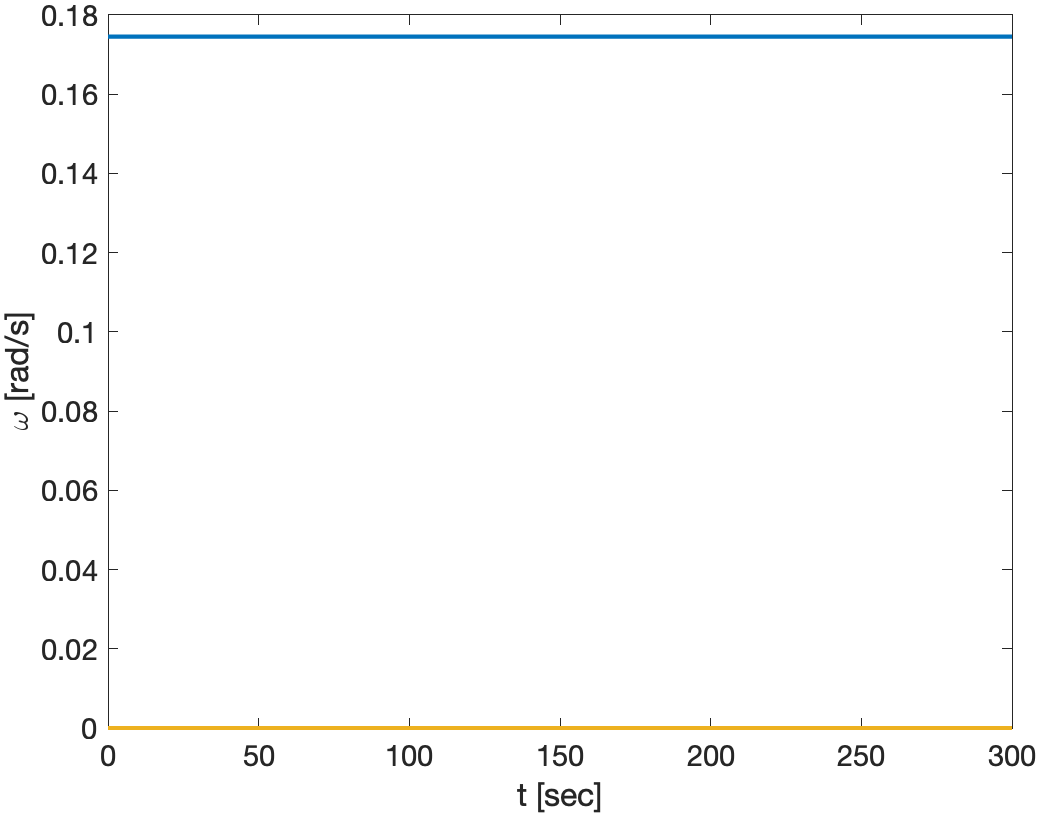
\includegraphics[width = 10cm]{Images/PS4/equilibrium_inertial_velocities.png}
    \caption{Angular Velocity Vector Components Expressed in the Principal Frame for Equilibrium about the Ineretial X-Axis}
    \label{fig:inertial_equilibrium_velocities}
\end{figure}

In Figure \ref{fig:inertial_equilibrium_velocities} it can be seen that the initial angular velocities are conserved for the full 300 second simulation. Primarily, $\omega_y$ and $\omega_z$ stay at zero.

\begin{figure}[H]
    \centering
    \captionsetup{justification = centering}
    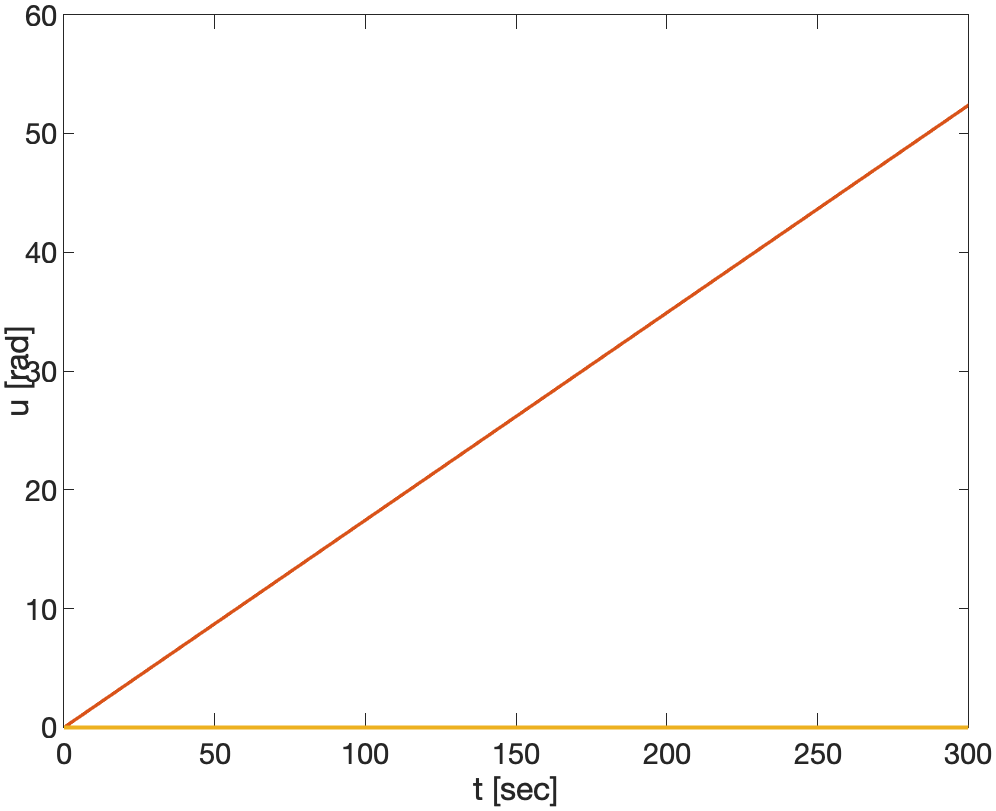
\includegraphics[width = 10cm]{Images/PS4/equilibrium_inertial_angles.png}
    \caption{312 Euler Angles Describing Rotation between Inertial and Principal Frame}
    \label{fig:inertial_equilibrium_angles}
\end{figure}

In Figure \ref{fig:inertial_equilibrium_angles}, it can be seen that $\psi$ and $\phi$ are zero for the full simulation and $\theta$ increases linearly which is consistent with the constant angular velocities.

\subsubsection{Repeat a. by setting the initial attitude to match the RTN frame. Set the initial angular velocity to
be non-zero only about N. Show the evolution of attitude motion in the RTN frame and give an
interpretation of the results (recall that you might have J2 effects in orbit propagation, consider
removing them for verification).}

To set the initial attitude to match the RTN frame, the initial position and velocity of the orbit was calculated in the ECI frame with the same orbital elements from Homework 2. From there the rotation matrix from ECI to RTN was found and then converted into Euler angles with the two functions shown below.

\begin{figure} [H]
    \centering
    \begin{lstlisting}
function u = RtoEuler312(R)

    u = zeros([3 1]);

    u(1) = atan2(R(1,2), R(2,2));
    u(2) = -asin(R(3,2));
    u(3) = atan2(R(3,1), R(3,3));

end

function R_eci_to_rtn = eci2rtn(r_eci, v_eci)
    
    % Compute radial, transverse, and normal vectors in ECI frame
    r_radial_eci = r_eci;
    r_normal_eci = cross(r_radial_eci, v_eci);
    r_transverse_eci = -cross(r_radial_eci, r_normal_eci);
    
    % Normalize radial, transverse, and normal vectors to obtain unit vectors
    r_radial_eci_unit = r_radial_eci / norm(r_radial_eci);
    r_transverse_eci_unit = r_transverse_eci / norm(r_transverse_eci);
    r_normal_eci_unit = r_normal_eci / norm(r_normal_eci);
    
    % Construct rotation matrix from ECI to RTN
    R_eci_to_rtn = [r_radial_eci_unit.'; r_transverse_eci_unit.'; r_normal_eci_unit.'];

end
    \end{lstlisting}
    \caption{Euler Angle RTN Alignment}
    \label{fig:euler_angle_prop_model}
\end{figure}

The Simulink model from Homework 3 was then used to propagate the initial conditions with the only modification being that a Simulink model was created to output the ECI to RTN DCM as the simulation was running as opposed to using a separate MATLAB script. This model is shown in Figures \ref{fig:orb_prop_simulink_num} and \ref{fig:orb_prop_simulink_kep} that show the two ways that the orbit could be propagated, Keplerian or Numerical methods.

\begin{figure}[H]
    \centering
    \captionsetup{ justification = centering}
    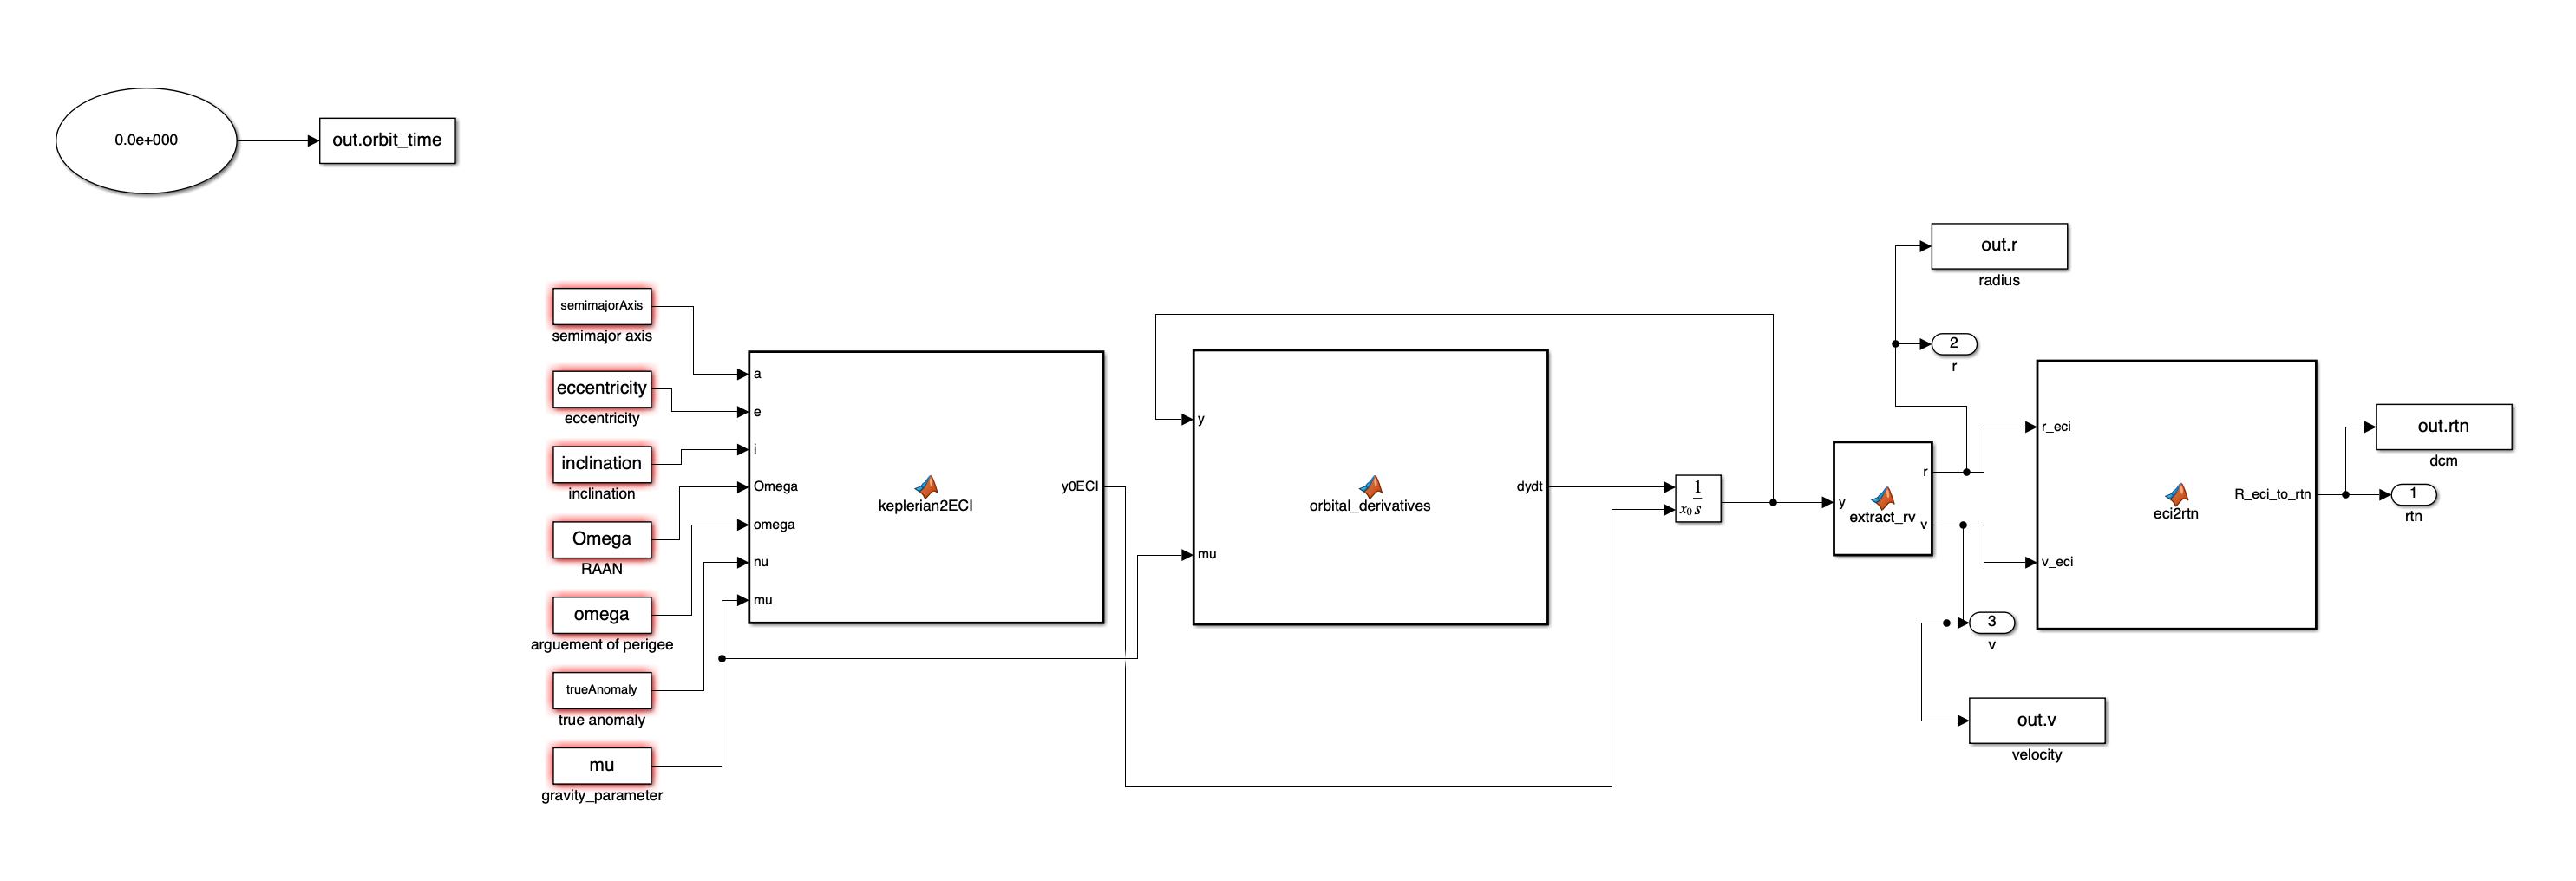
\includegraphics[width = 15cm]{Images/PS4/orbital_prop_simulink_num.png}
    \caption{Numerical Orbit Propagator Simulink Model}
    \label{fig:orb_prop_simulink_num}
\end{figure}

\begin{figure}[H]
    \centering
    \captionsetup{ justification = centering}
    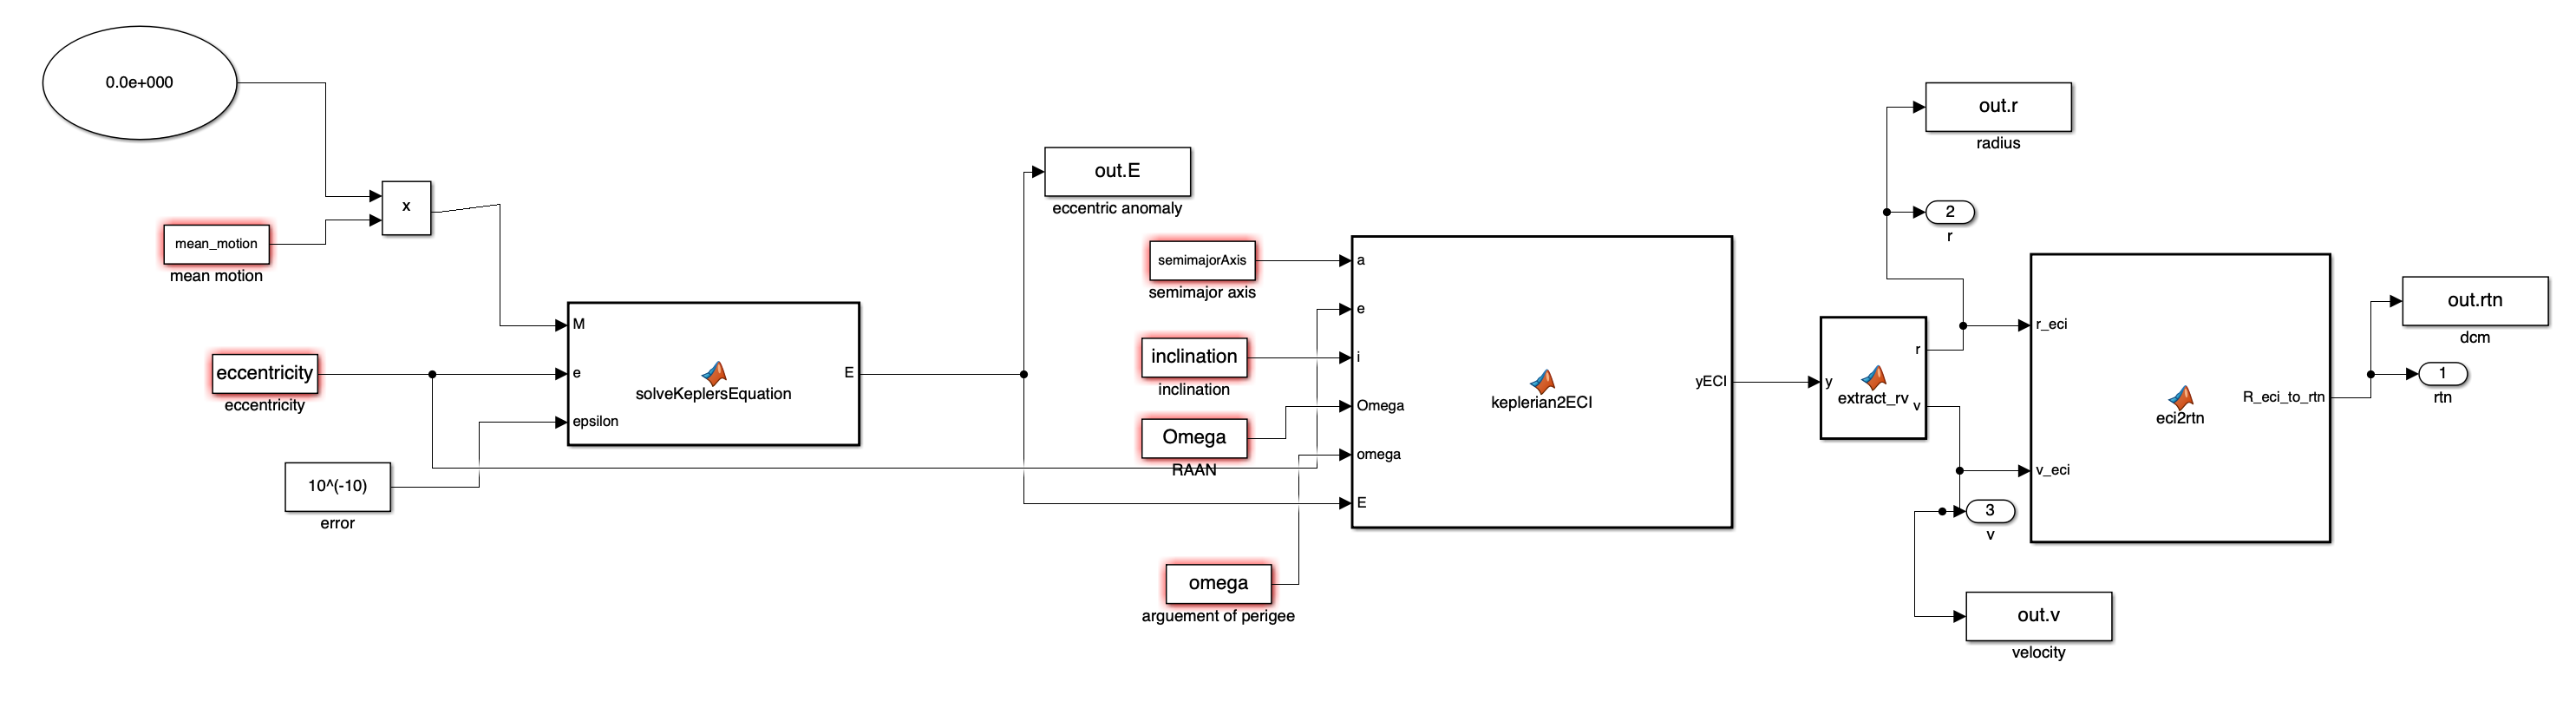
\includegraphics[width = 15cm]{Images/PS4/orbital_prop_simulink_kep.png}
    \caption{Keplerian Orbit Propagator Simulink Model}
    \label{fig:orb_prop_simulink_kep}
\end{figure}

Using this model, Figures \ref{fig:RTN_equilibrium_velocities} and \ref{fig:RTN_equilibrium_angles} were created.


\begin{figure}[H]
    \centering
    \captionsetup{ justification = centering}
    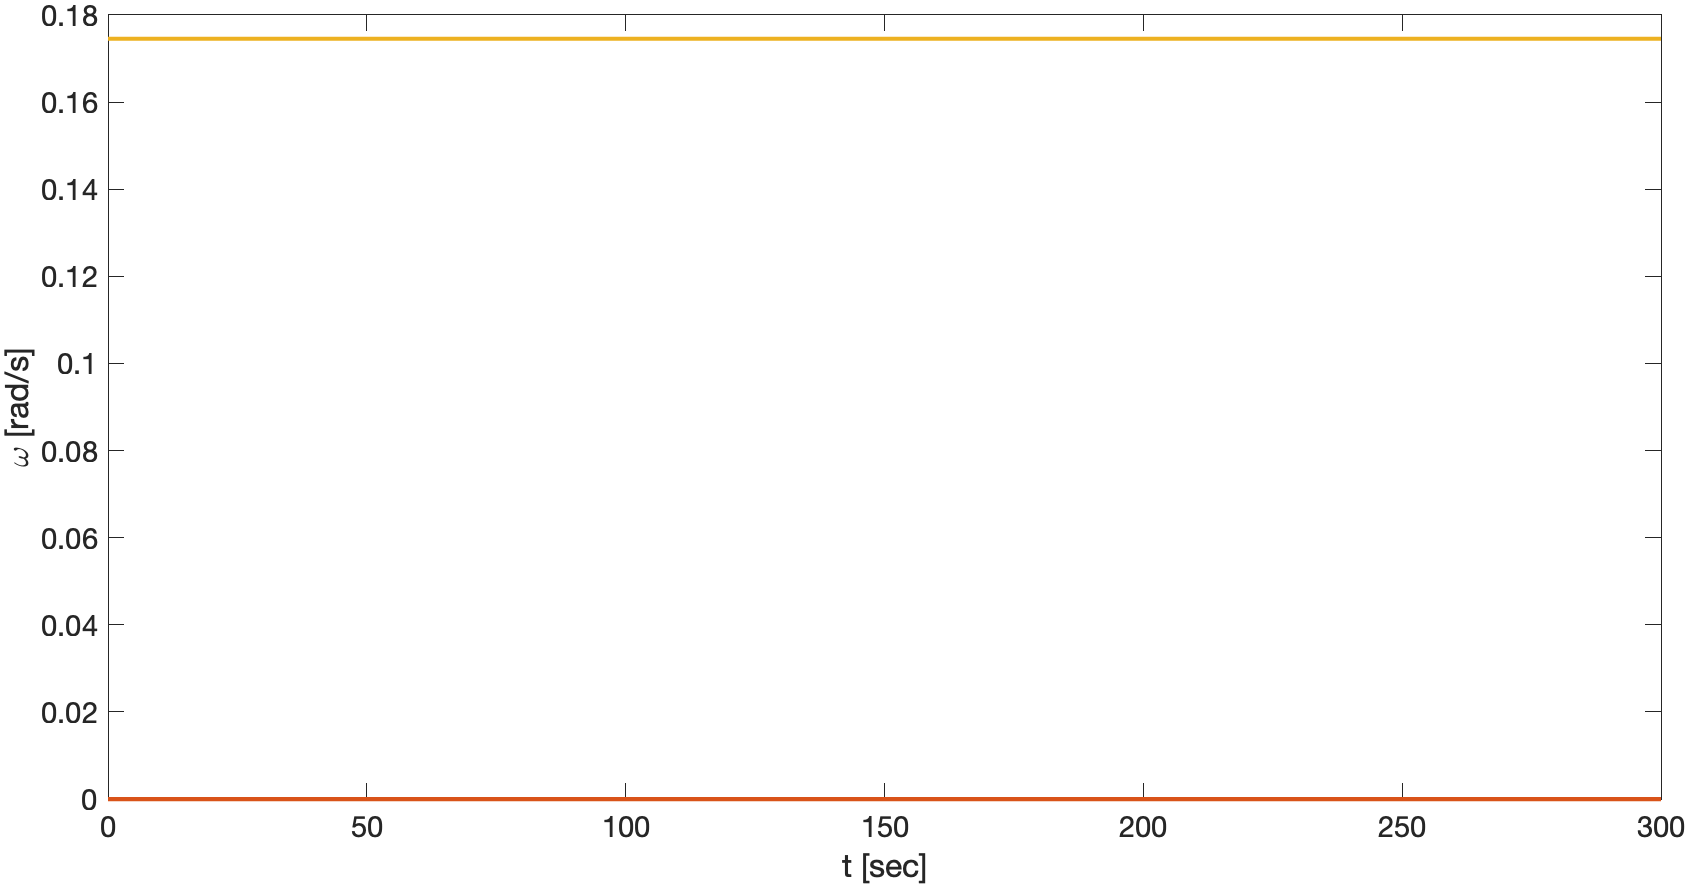
\includegraphics[width = 10cm]{Images/PS4/equilibrium_RTN_velocities.png}
    \caption{Angular Velocity Vector Components Expressed in the Principal Frame for Equilibrium about N-Axis}
    \label{fig:RTN_equilibrium_velocities}
\end{figure}

\begin{figure}[H]
    \centering
    \captionsetup{justification = centering}
    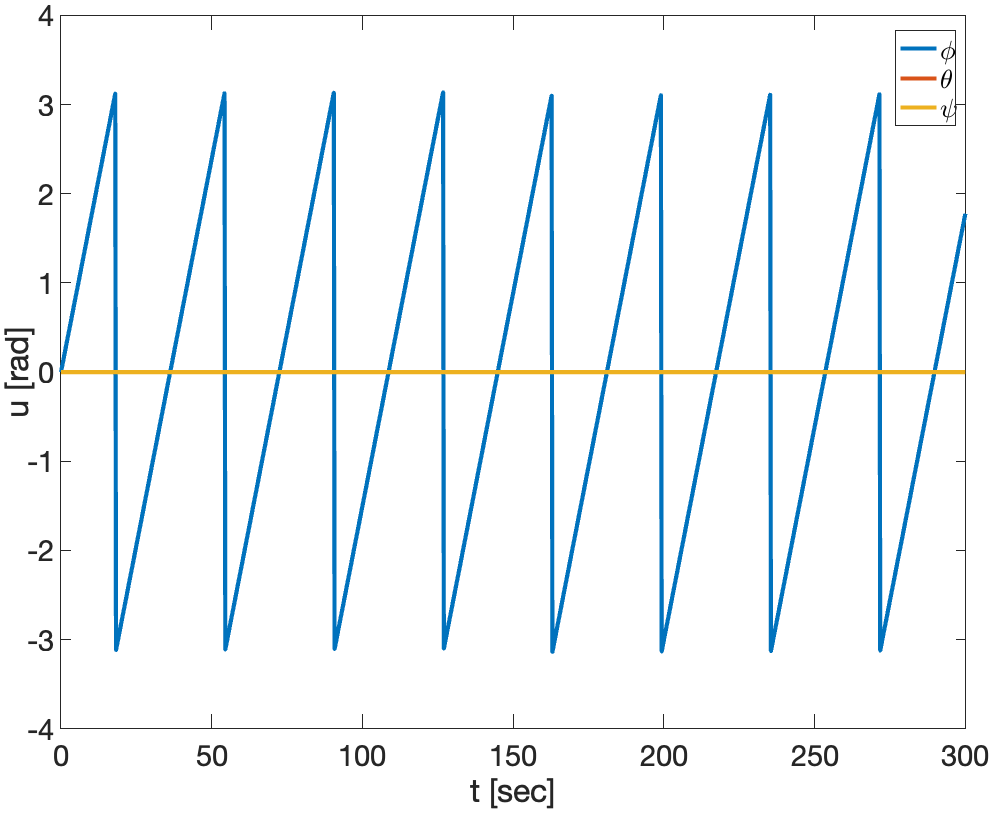
\includegraphics[width = 10cm]{Images/PS4/equilibrium_RTN_angles.png}
    \caption{312 Euler Angles Describing Rotation between RTN and Principal Frame}
    \label{fig:RTN_equilibrium_angles}
\end{figure}

In Figure \ref{fig:RTN_equilibrium_velocities} it can be seen that the angular velocities were once again constant, and in Figure \ref{fig:RTN_equilibrium_angles} it can be seen that the satellite only rotated about $\phi$ at a constant rate (note that the maximum and minimum angles were capped at $\pi$ and $-\pi$). Note that this equilibrium point yields these results due to the N direction in the RTN frame remaining constant. That is, the orbital plane is not changing, therefore pure rotations about that axis will yield linearly increasing Euler angles just as was seen in the inertial frame.

\subsection{Problem 2 - Stability Tests}

\subsubsection{Pretend you have a single-spin satellite. Set initial conditions to correspond alternatively to the 3
possible equilibrium configurations (rotation about principal axes of inertia). Slightly perturb initial
condition. Is the attitude stable or unstable? In angles and velocities? If stable, periodically or
asymptotically? Show it.}

To perturb the three possible equilibrium positions, the same simulation from Problem 1 was run three times with the primary rotation axis being permuted for each simulation with all states being offset by randomly generated numbers. The attitude state reperesented in Euler angles was also randomly perturbed. From this, Figures \ref{fig:stability_velocities} and \ref{fig:stability_angles} were created to shown the time histories of the perturbed angular velocities and Euler angles.

\begin{figure}[H]
    \centering
    \captionsetup{ justification = centering}
    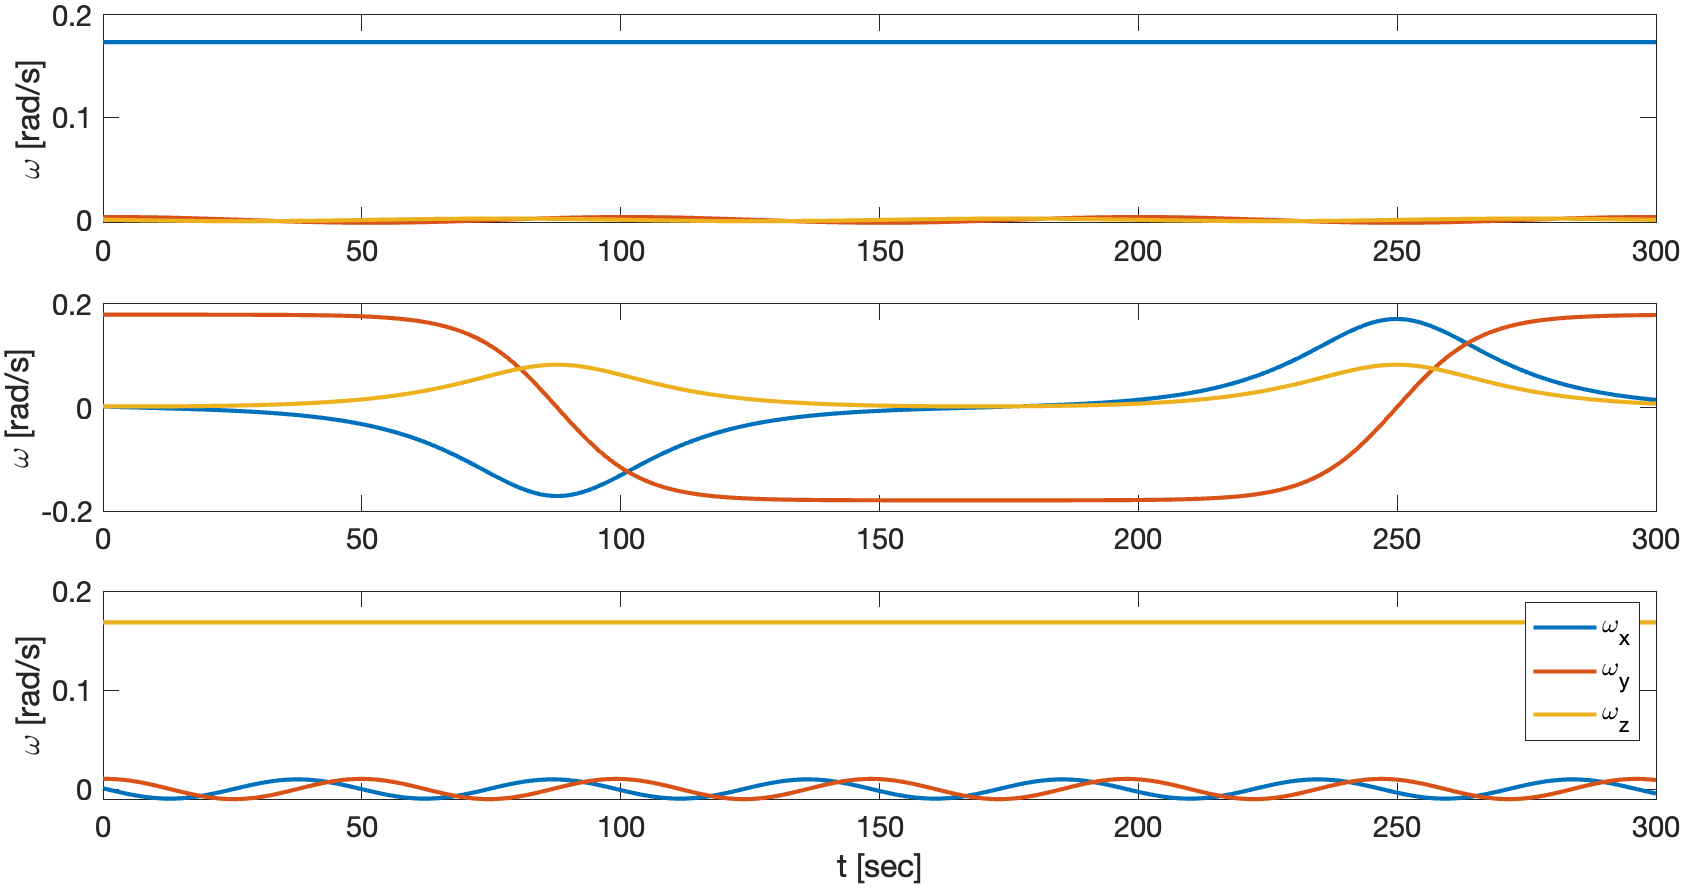
\includegraphics[width = 10cm]{Images/PS4/stability_history_velocity.png}
    \caption{Time History of Perturbed Angular Velocity Vector Components Expressed in Principal Frame}
    \label{fig:stability_velocities}
\end{figure}

\begin{figure}[H]
    \centering
    \captionsetup{justification = centering}
    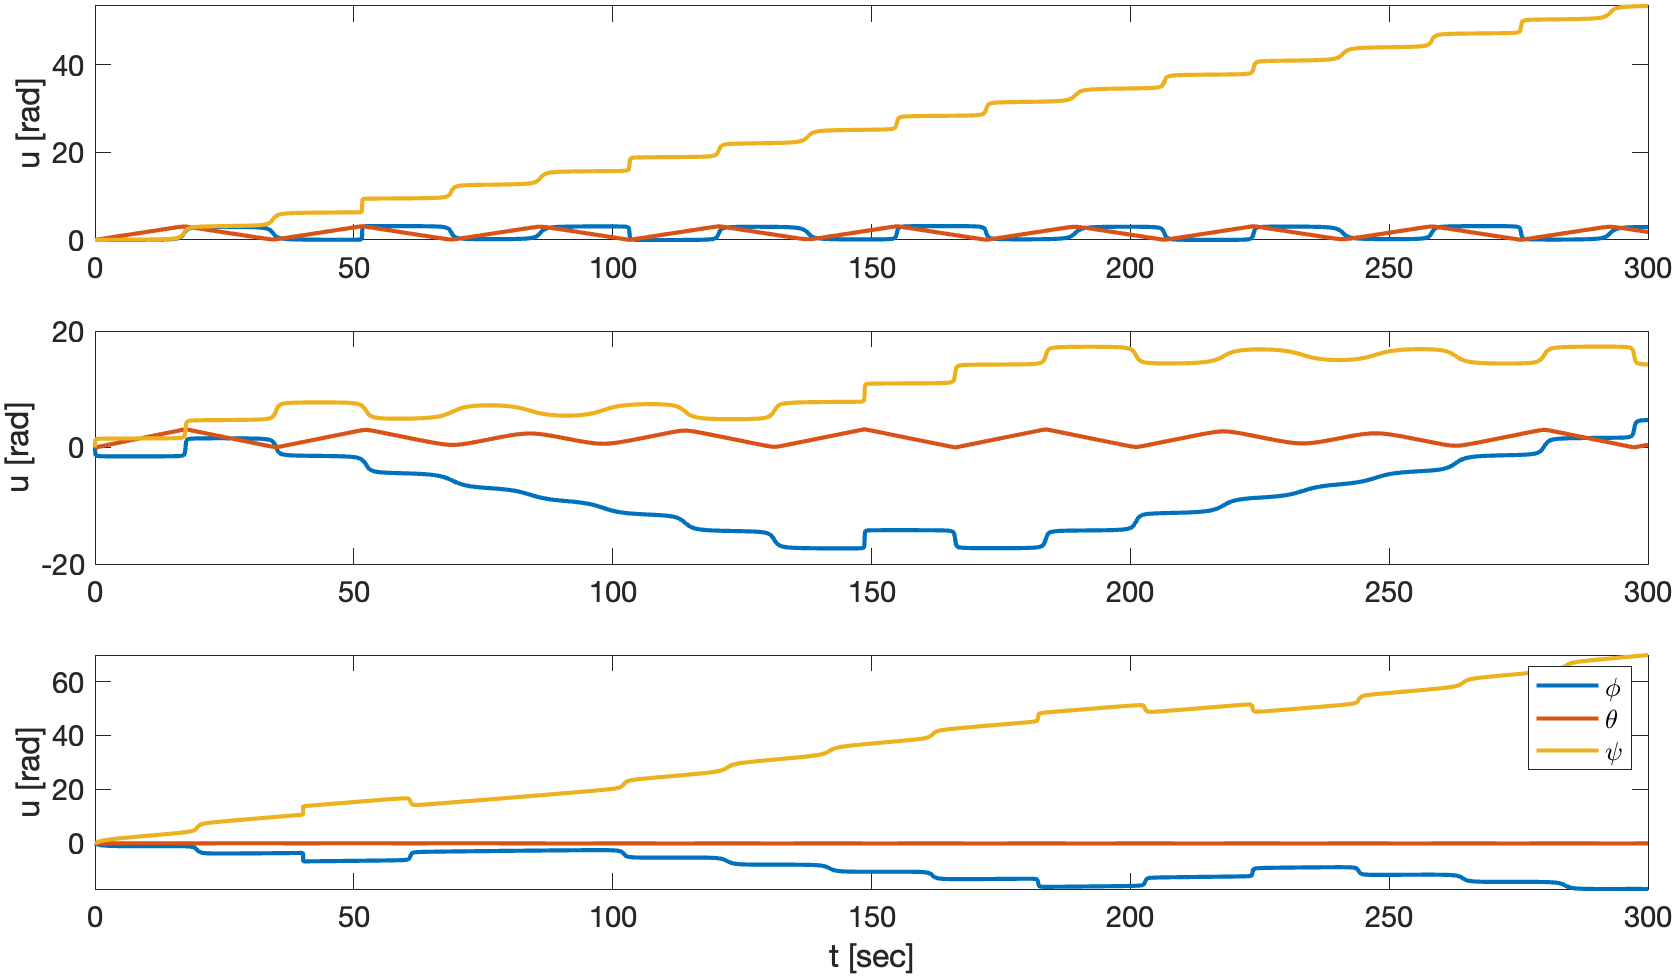
\includegraphics[width = 10cm]{Images/PS4/stability_history_angles.png}
    \caption{Time History of Perturbed 312 Euler Angles Describing Rotation between Inertial and Principal Frame}
    \label{fig:stability_angles}
\end{figure}

From these figures, it can be seen that when perturbing $\omega_x$ and $\omega_z$, the solutions were periodically stable. However, when perturbing $\omega_y$ the solutions were unstable and varied greatly across the simulation. This aligns with the theory supporting that asymptotic stability can be achieved for the maximum and minimum moments of inertia along the principle axes, but not the intermediate. This result is theoretically proved through taking the equilibrium points of the Euler equations for a single-spin satellite and linearizing them through taking small perturbations of the equilibrium. The resultant linear equations are shown below.

\begin{equation}
    I_x \dot \omega_x + (I_z - I_y) (\omega_y \bar{\omega}_z ) = 0
\end{equation}
\begin{equation*}
        I_y \dot \omega_y + (I_x - I_z) (\omega_x \bar{\omega}_z ) = 0
\end{equation*}
\begin{equation*}
        I_z \dot \omega_z = 0
\end{equation*}

Through finding the eigenvalues of this system and determining what conditions make them zero, it can be seen that they're only stable when $(I_y - I_z)(I_z - I_x) < 0$. This is not the case, as can be seen in Section \ref{sec:principal_inertia_def_and_calc} where $I_x < I_y < I_z$.

\subsection{Problem 3 - Adding a Momentum Wheel or Rotor (Dual-Spin Satellite)}

\subsubsection{Re-program Euler equations to include a generic momentum wheel or rotor with rotation axis
aligned with one of the principal axes of inertia. Ideally the wheel or rotor has specs representative
of commercial products (inertia, rotational speed).}

Dual-spin satellites solve several of the problems with single-spin satellites including limitations in size and what rotations are possible. Dual-spin satellites use a momentum wheel or rotor that rotates around a desired axis. Furthermore, passive stabilization is possible for a dual-spin satellite unlike with a single-spin satellite.

With the addition of the momentum wheel, the angular momentum vector of the satellite becomes a sum of the original vector (without the momentum wheel) and that of the momentum wheel. This can be used to rewrite the Euler equations with additional terms for the momentum wheel. These modified equations are shown below after assuming that $\omega_r$ is constant and solving for $\dot \omega$.

\begin{equation}
\dot \omega_x = \frac{1}{I_x} \left[M_x - (I_z - I_y)\omega_y \omega_z - I_r \omega_r (\omega_y r_z - \omega_z r_y) \right]
\end{equation}

\begin{equation*}
\dot \omega_y = \frac{1}{I_y} \left[M_y - (I_x - I_z)\omega_z \omega_x - I_r \omega_r (\omega_z r_x - \omega_x r_z) \right]
\end{equation*}

\begin{equation*}
\dot \omega_z = \frac{1}{I_z} \left[M_z - (I_y - I_x)\omega_x \omega_y - I_r \omega_r (\omega_x r_y - \omega_y r_x) \right]
\end{equation*}

A momentum wheel was added to the Euler angle propagator through the simulink model shown below in Figure \ref{fig:dual_spin_simulink}. Additionally, the script used in the simulink model is shown below in Figure \ref{fig:dual_spin_simulink_code}.

\begin{figure} [H]
    \centering
    \captionsetup{justification = centering}
    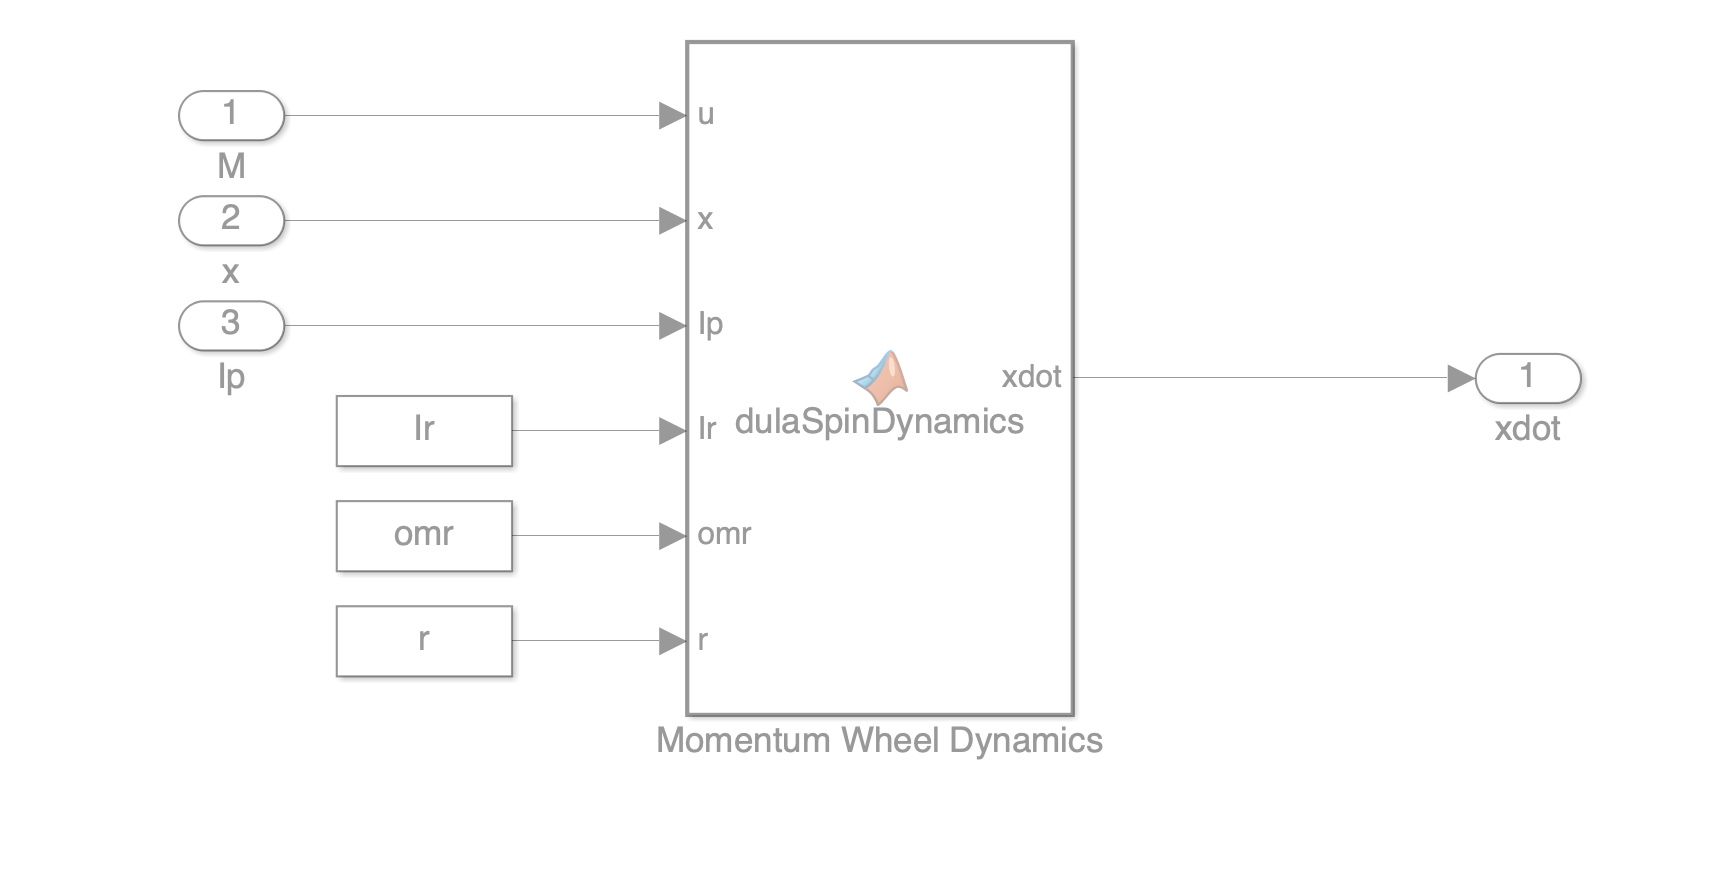
\includegraphics[width = 10cm]{Images/PS4/dualspin_simulink.png}
    \caption{Simulink Model to Account for Momentum Wheel in Euler Equations}
    \label{fig:dual_spin_simulink}
\end{figure}

\begin{figure} [H]
    \centering
    \begin{lstlisting}
function xdot = dualSpinDynamics(u,x,Ip,Ir,omr,r)

xdot = zeros(size(x));


Mx = u(1);
My = u(2);
Mz = u(3);

omx = x(1);
omy = x(2);
omz = x(3);

Ix = Ip(1,1);
Iy = Ip(2,2);
Iz = Ip(3,3);

rx = r(1);
ry = r(2);
rz = r(3);

wxdot = (1/Ix)*(Mx - ((Iz - Iy)*omy*omz + Ir*omr*(omy*rz - omz*ry)));
wydot = (1/Iy)*(My - ((Ix - Iz)*omz*omx + Ir*omr*(omz*rx - omx*rz)));
wzdot = (1/Iz)*(Mz - ((Iy - Ix)*omx*omy + Ir*omr*(omx*ry - omy*rx)));

xdot(1) = wxdot;
xdot(2) = wydot;
xdot(3) = wzdot;

end
    \end{lstlisting}
    \caption{Euler Angle Dual Spin Dynamics}
    \label{fig:dual_spin_simulink_code}
\end{figure}

\subsubsection{Numerically integrate Euler AND Kinematic equations from equilibrium initial condition. Verify
that integration is correct as from previous tests (conservation laws, rotations, etc.).}

To verify the integration, conservation of angular momentum was used. This was done by giving an initial angular velocity in all three of the inertial directions and plotting angular momentum to confirm that it remained constant throughout the integration. The results are shown below in Figure \ref{fig:mom_wheel_momentum_conservation}.

\begin{figure}[H]
    \centering
    \captionsetup{justification = centering}
    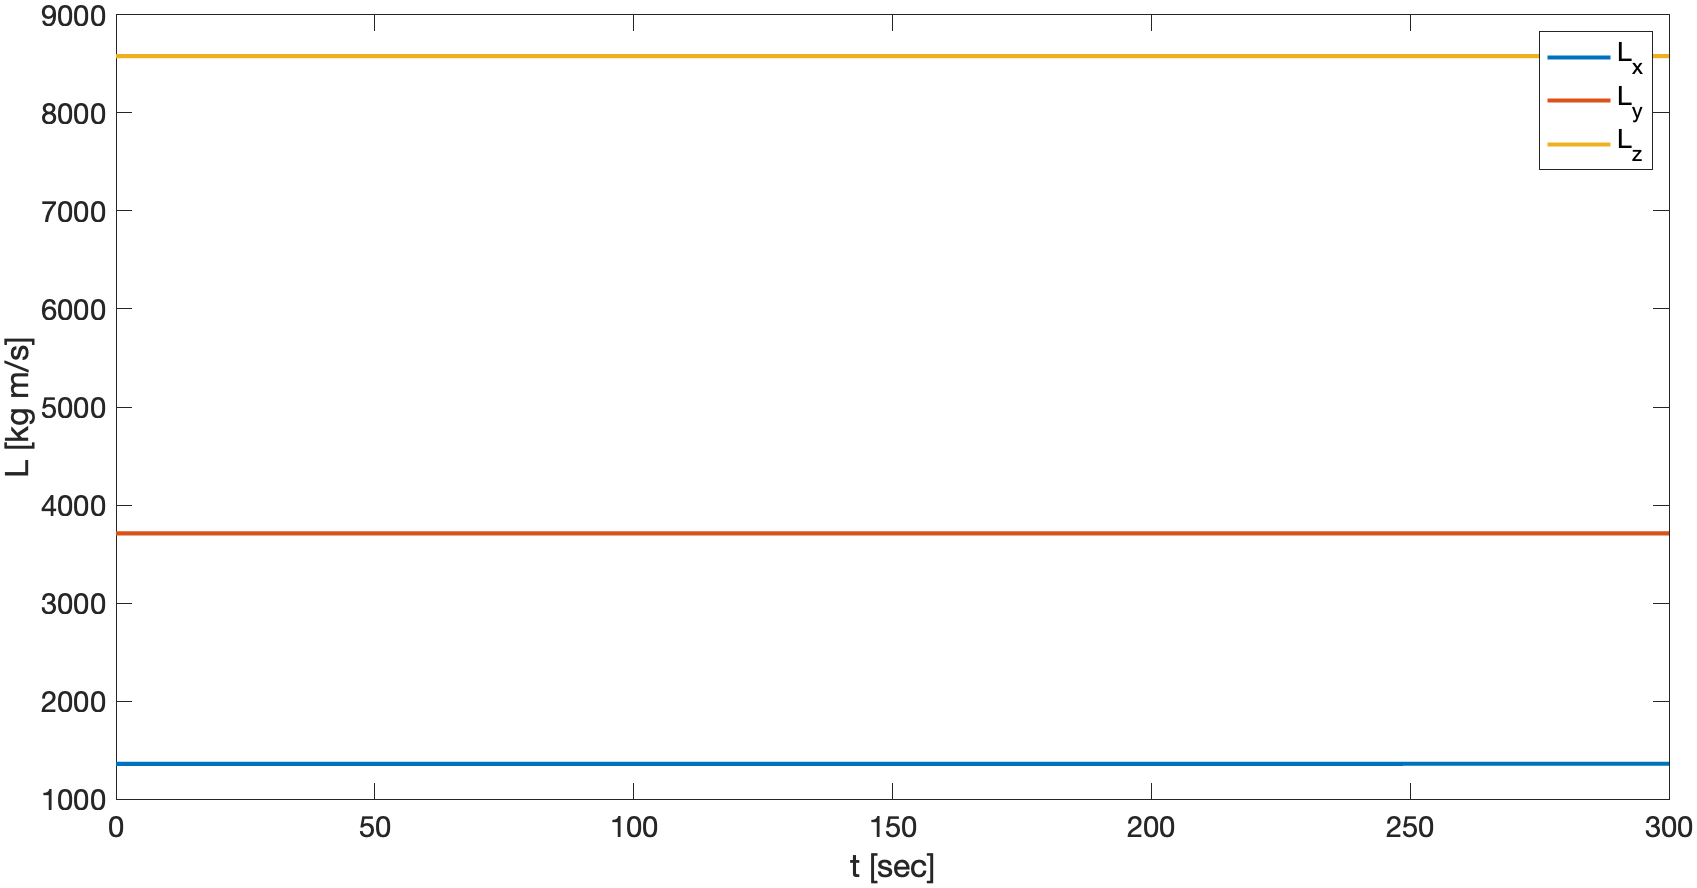
\includegraphics[width = 10cm]{Images/mom_wheel_angular_momentum.png}
    \caption{Angular Momentum Vector Components Represented in the Inertial Frame Plotted over Time}
    \label{fig:mom_wheel_momentum_conservation}
\end{figure}

In Figure \ref{fig:mom_wheel_momentum_conservation}, it can be seen that angular momentum was conserved in all three of the inertial directions, thus validating the new integration scheme for the momentum wheel.

\subsubsection{Verify equilibrium and its stability similar to previous pset.}

Just like in problem 1, the initial Euler angles were first aligned with the inertial frame to obtain results shown in Figures \ref{fig:mom_wheel_inertial_equilibrium} and \ref{fig:mom_wheel_equilibrium_inertial_angles}.

\begin{figure}[H]
    \centering
    \captionsetup{justification = centering}
    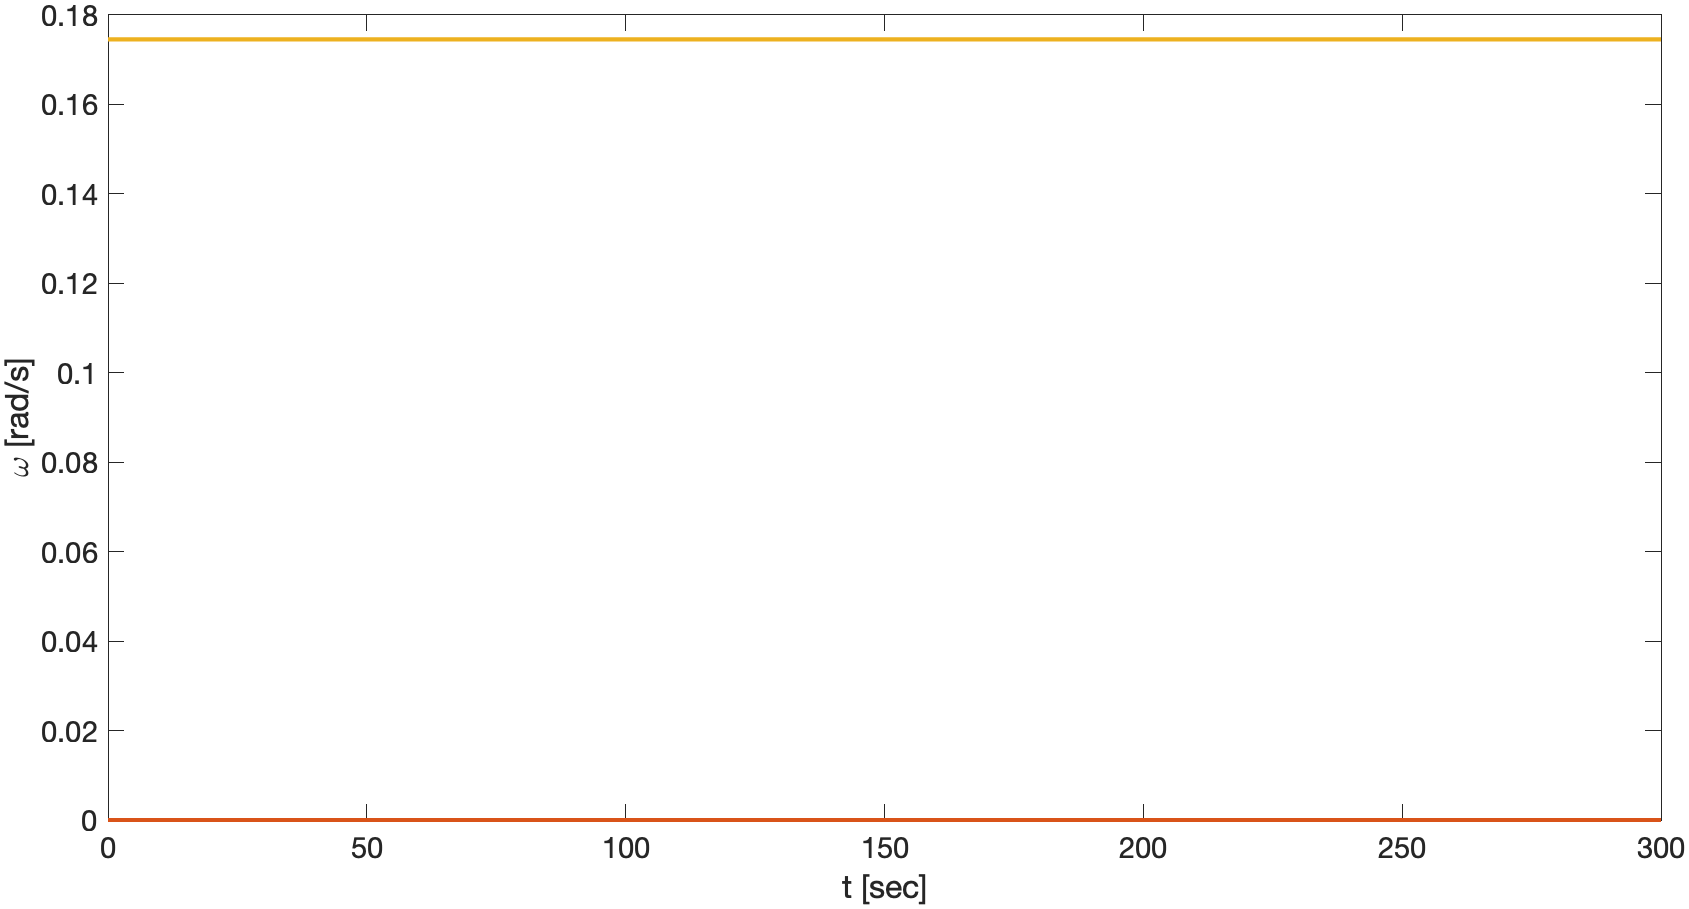
\includegraphics[width = 10cm]{Images/PS4/mom_wheel_equilibrium_inertial_velocities.png}
    \caption{Angular Velocity Vector Components Expressed in the Principal Frame for Equilibrium about the Inertial Z-Axis}
    \label{fig:mom_wheel_inertial_equilibrium}
\end{figure}

\begin{figure}[H]
    \centering
    \captionsetup{justification = centering}
    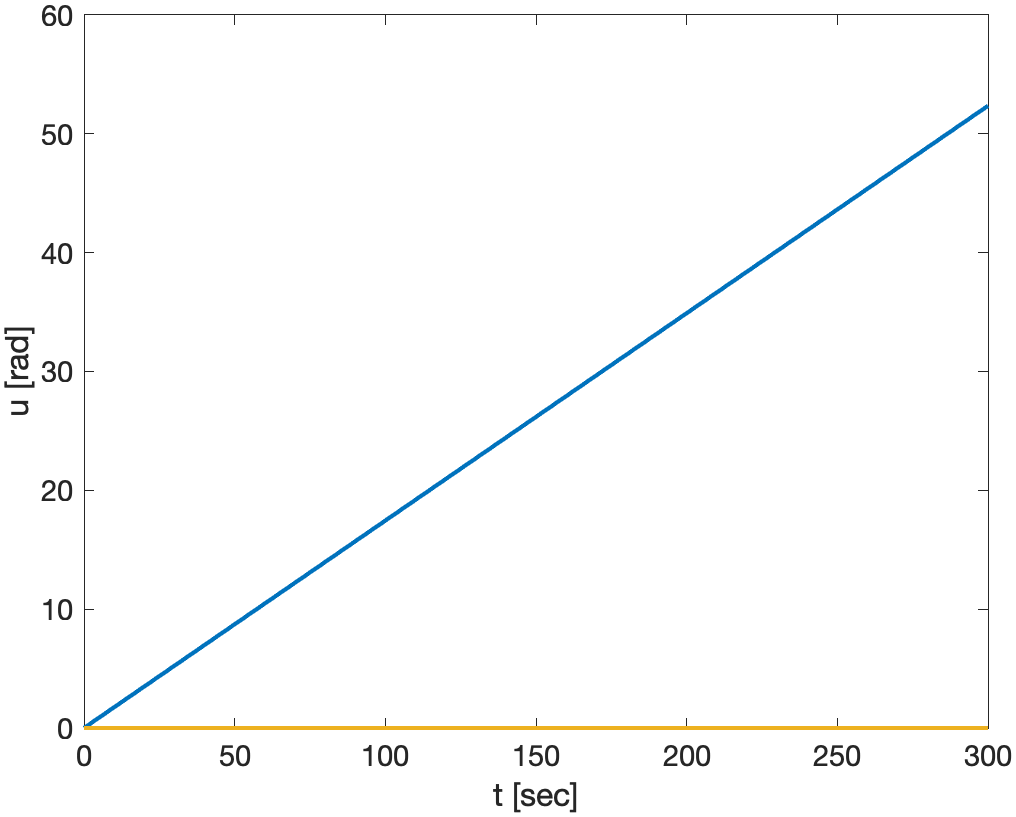
\includegraphics[width = 10cm]{Images/PS4/mom_wheel_equilibrium_inertial_angles.png}
    \caption{312 Euler Angles Describing Rotation between Inertial and Principal Frame}
    \label{fig:mom_wheel_equilibrium_inertial_angles}
\end{figure}

Figures \ref{fig:mom_wheel_inertial_equilibrium} and \ref{fig:mom_wheel_equilibrium_inertial_angles} show that once again the angular velocity vector components remained constant and the rotation between the inertial and principal frames only happened in $\omega_z$.

Next, the initial Euler angles were aligned with the RTN frame through the same procedure shown in problem 1 to obtain Figures \ref{fig:mom_wheel_RTN_equilibrium} and \ref{fig:mom_wheel_equilibrium_RTN_angles}.

\begin{figure}[H]
    \centering
    \captionsetup{justification = centering}
    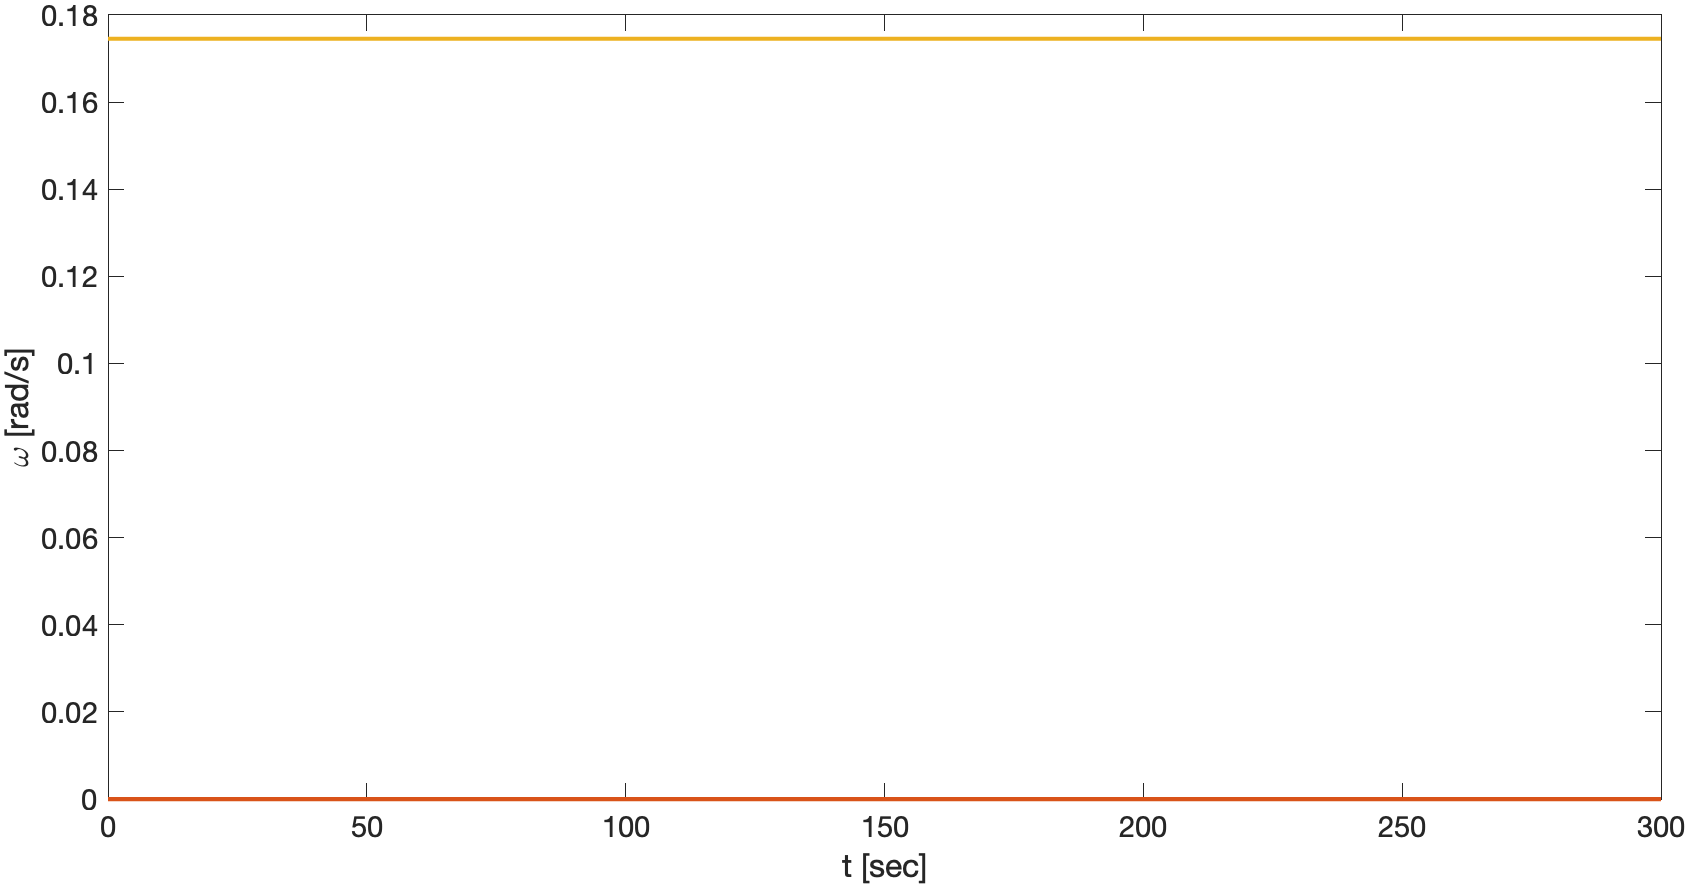
\includegraphics[width = 10cm]{Images/PS4/mom_wheel_equilibrium_RTN_velocities.png}
    \caption{Angular Velocity Vector Components Expressed in the Principal Frame for Equilibrium about the N-Axis}
    \label{fig:mom_wheel_RTN_equilibrium}
\end{figure}

\begin{figure}[H]
    \centering
    \captionsetup{justification = centering}
    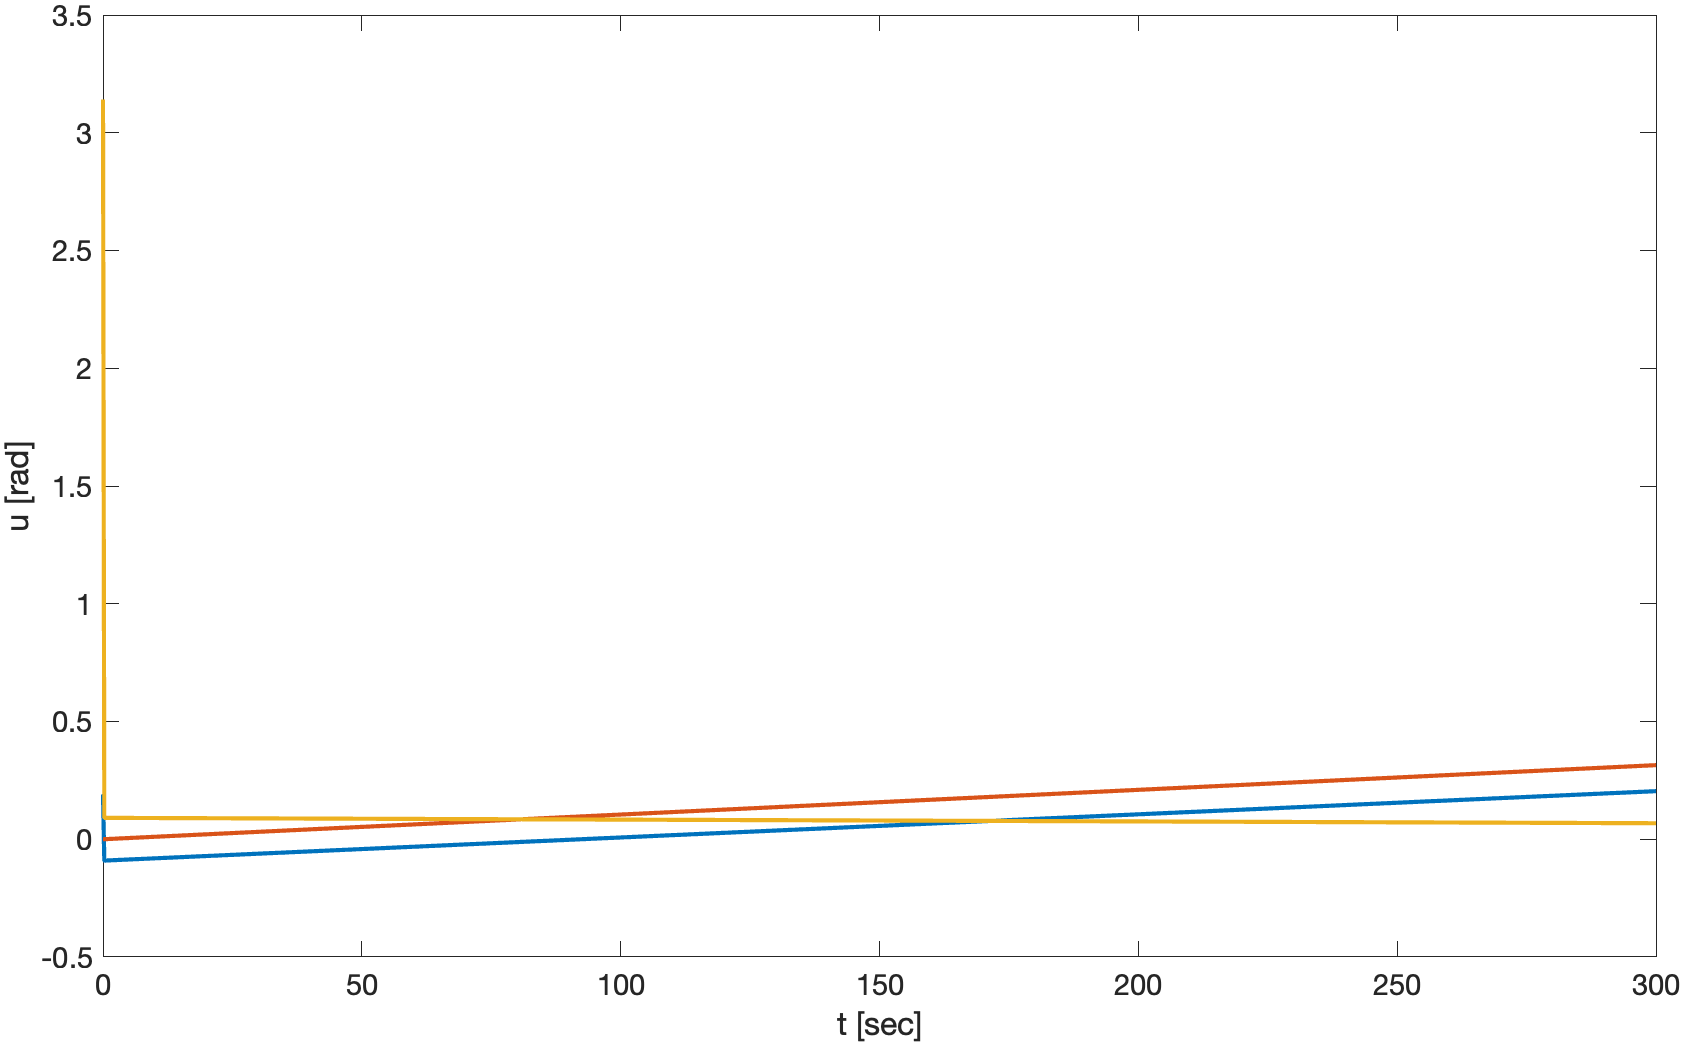
\includegraphics[width = 10cm]{Images/PS4/mom_wheel_equilibrium_RTN_angles.png}
    \caption{312 Euler Angles Describing Rotation between RTN and Principal Frame}
    \label{fig:mom_wheel_equilibrium_RTN_angles}
\end{figure}

Figures \ref{fig:mom_wheel_RTN_equilibrium} and \ref{fig:mom_wheel_equilibrium_RTN_angles} show that equilibrium about the N-Axis was once again achieved through having zero angular velocity in the other two directions. Additionally, the Euler angles only rotated about $\omega_z$ between the two frames.

The same procedure of using randomly perturbed initial conditions was used for the momentum stability test. Through selecting random initial conditions for the Euler angles and angular velocities, Figures \ref{fig:mom_wheel_stability_velocities} and \ref{fig:mom_wheel_stability_angles} were created.

\begin{figure}[H]
    \centering
    \captionsetup{ justification = centering}
    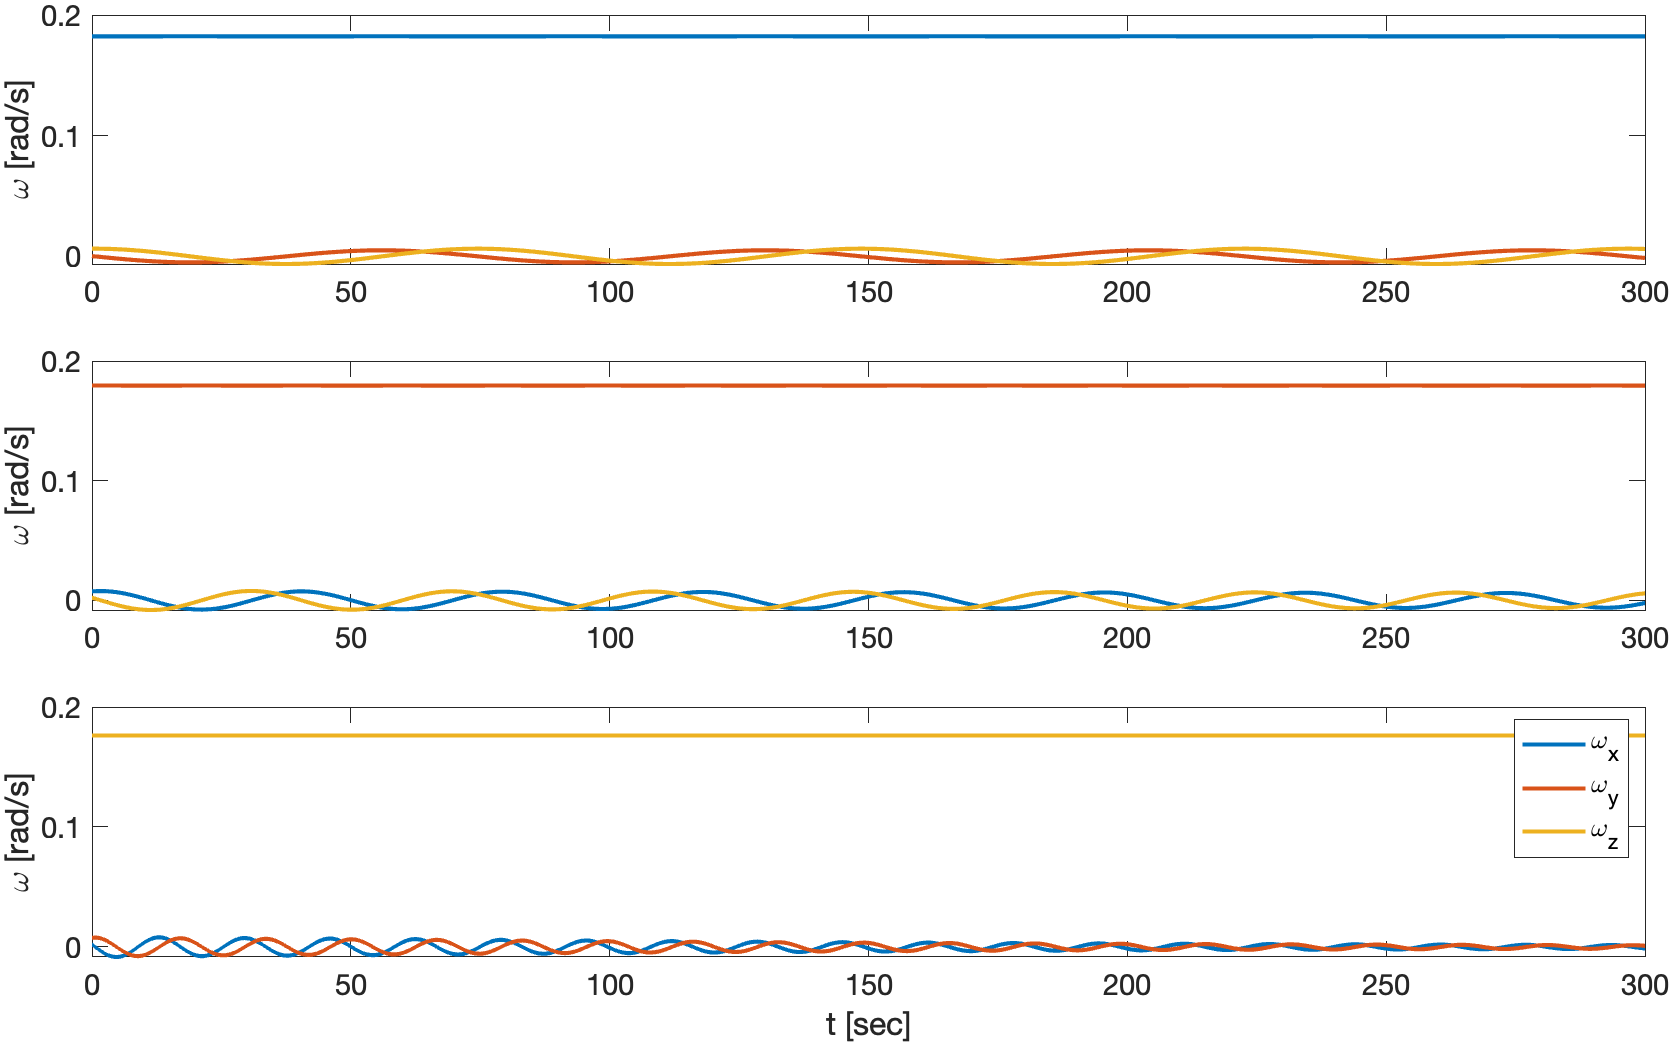
\includegraphics[width = 10cm]{Images/PS4/mom_wheel_stability_history_velocity.png}
    \caption{Time History of Perturbed Angular Velocity Vector Components Expressed in Principal Frame}
    \label{fig:mom_wheel_stability_velocities}
\end{figure}

\begin{figure}[H]
    \centering
    \captionsetup{justification = centering}
    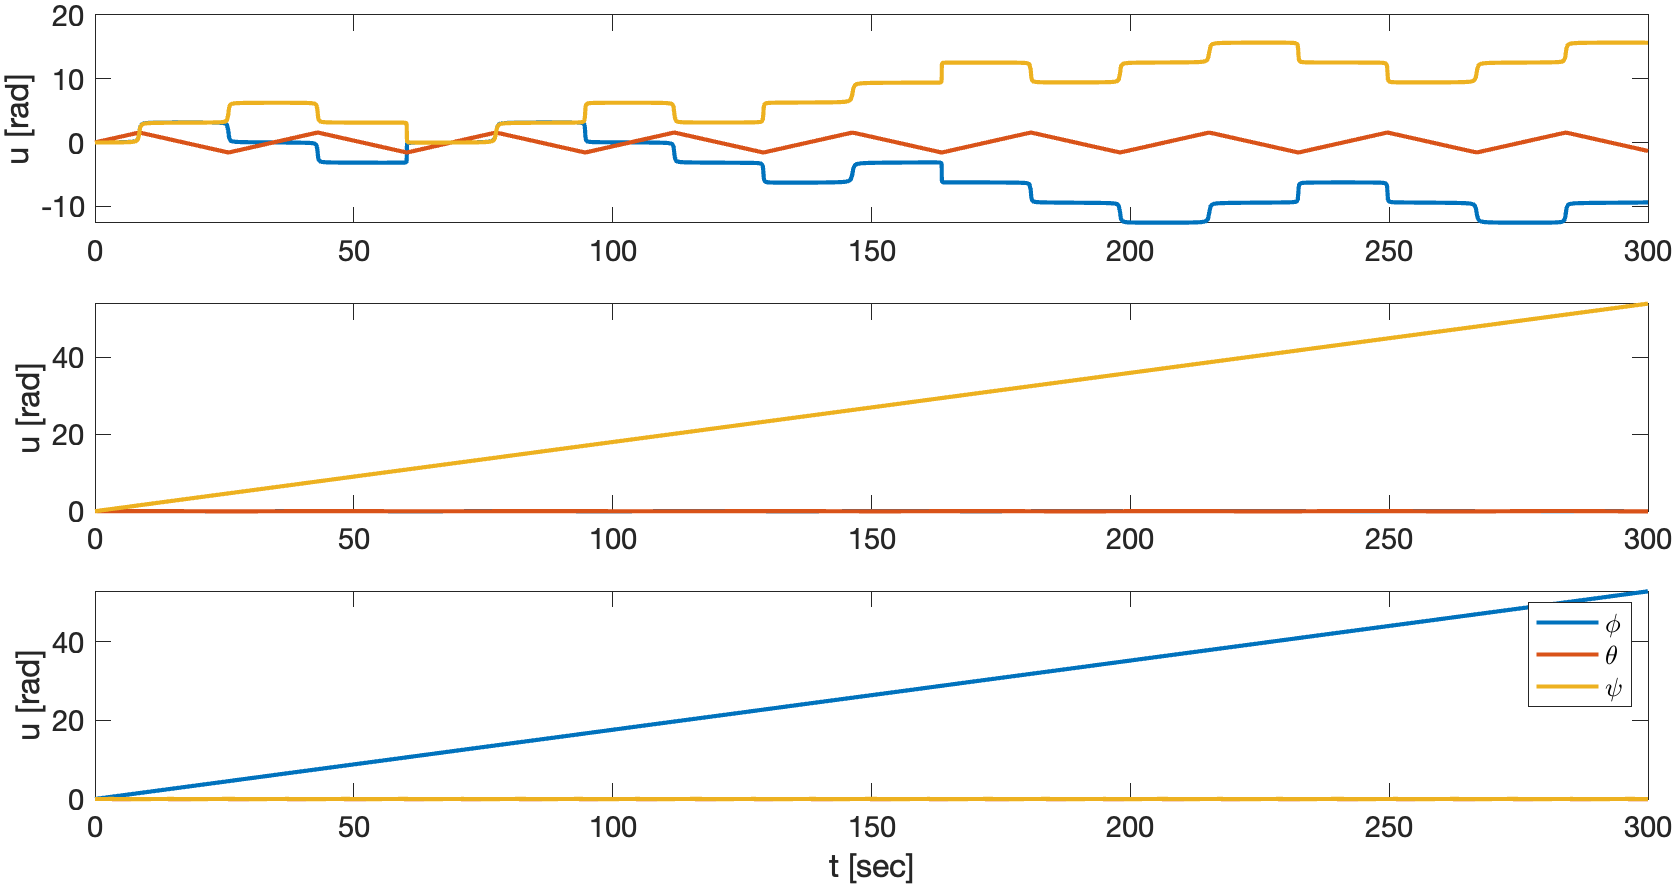
\includegraphics[width = 10cm]{Images/PS4/mom_wheel_stability_history_angles.png}
    \caption{Time History of Perturbed 312 Euler Angles Describing Rotation between Inertial and Principal Frame}
    \label{fig:mom_wheel_stability_angles}
\end{figure}

Figures \ref{fig:mom_wheel_stability_velocities} and \ref{fig:mom_wheel_stability_angles} show that once again, the angular velocities and Euler angles were stable in two of the three axes. 

\subsubsection{Use the stability condition to make attitude motion stable for rotation about intermediate moment of inertia by changing moment of inertia and/or angular velocity of the momentum wheel or rotor.}

Through once again taking the equilibrium values of the Euler equations for a satellite and rotor, perturbing, and linearizing them, the following equations for the linear system can be obtained.

\begin{equation}
    I_x \dot \omega_x + \left [ (I_z - I_y) \bar{\omega}_z + I_r \bar{\omega}_r \right] \omega_y = 0
\end{equation}

\begin{equation*}
    I_y \dot \omega_y + \left [ (I_x - I_z) \bar{\omega}_z - I_r \bar{\omega}_r \right] \omega_x = 0
\end{equation*}

Taking the eigenvalues of this linear system yields the following two stability conditions.

\begin{align} \label{eq:stability_cond_rotor}
    I_r \bar{\omega}_r > (I_y - I_z) \bar{\omega}_z && I_r \bar{\omega}_r > (I_x - I_z) \bar{\omega}_z \\
    \label{eq:stability_cond_rotor_two}
    I_r \bar{\omega}_r < (I_y - I_z) \bar{\omega}_z && I_r \bar{\omega}_r < (I_x - I_z) \bar{\omega}_z
\end{align}

If the both of the stability equations in Equation \ref{eq:stability_cond_rotor} or Equation \ref{eq:stability_cond_rotor_two} are met, the satellite can be stabilized with zero spin ($\bar{\omega}_z = 0$). For our implementation, we varied the moment of inertia and angular velocity of the rotor until $\omega_x$ and $\omega_z$ were asymptotically stable around zero and $\omega_y$ was constant, a configuration that wasn't possible for a single spin satellite.

\begin{figure}[H]
    \centering
    \captionsetup{ justification = centering}
    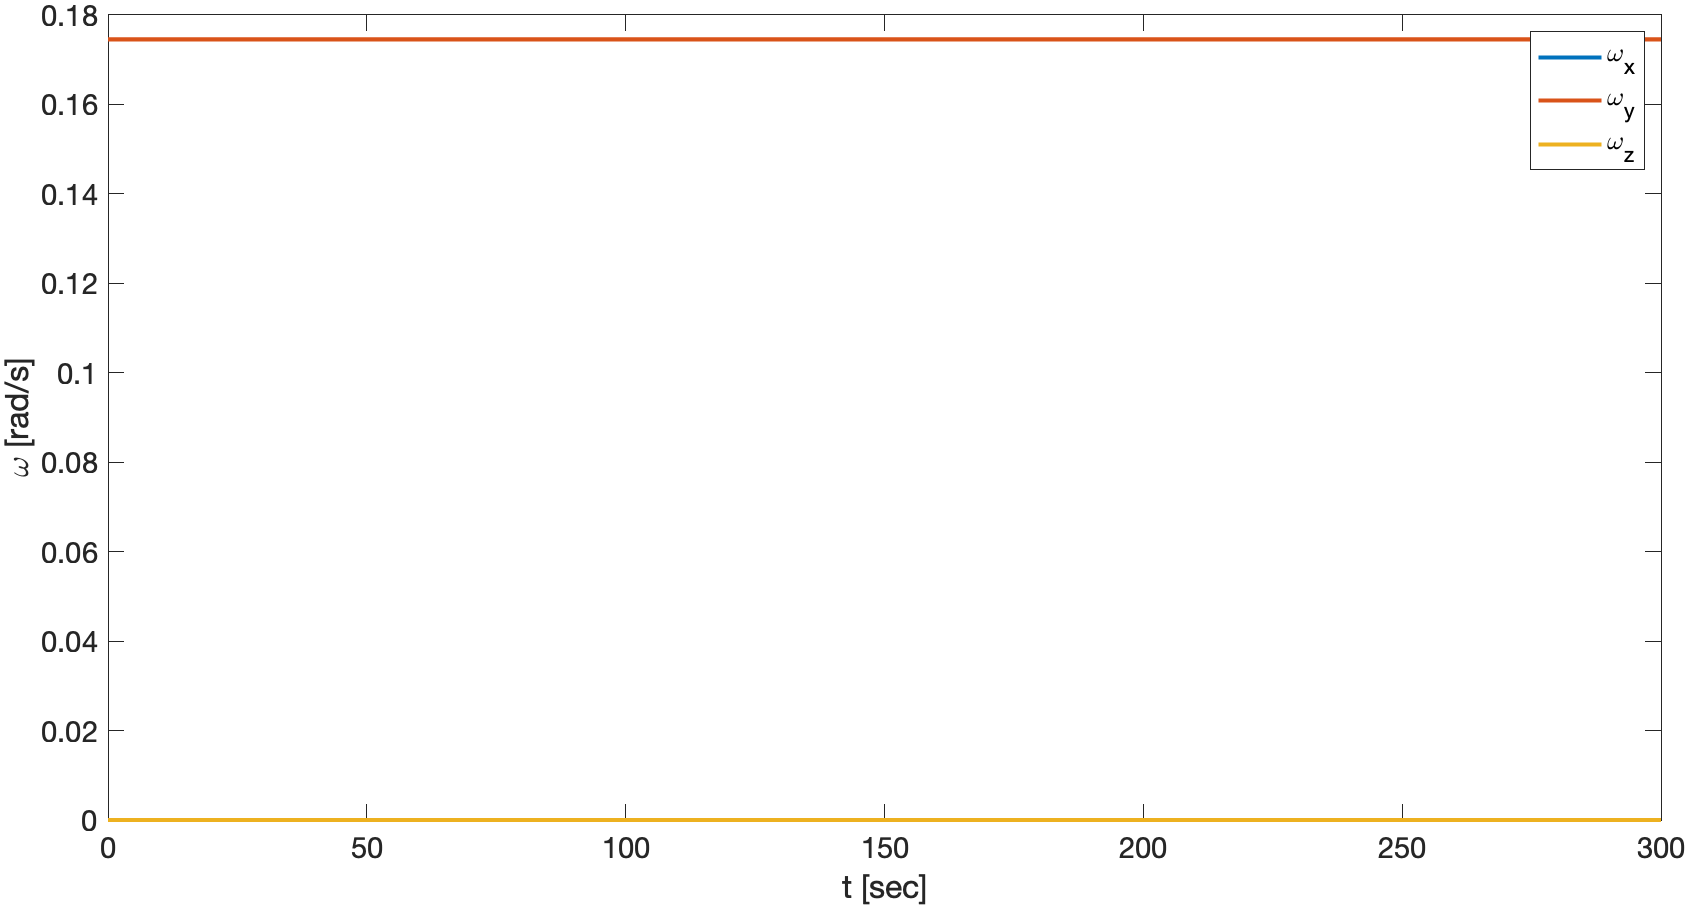
\includegraphics[width = 10cm]{Images/PS4/mom_wheel_intermediate_stability_history_velocity.png}
    \caption{Time History of Perturbed Angular Velocity Vector Components Expressed in Principal Frame}
    \label{fig:mom_wheel_intermediate_stability_velocities}
\end{figure}

\begin{figure}[H]
    \centering
    \captionsetup{justification = centering}
    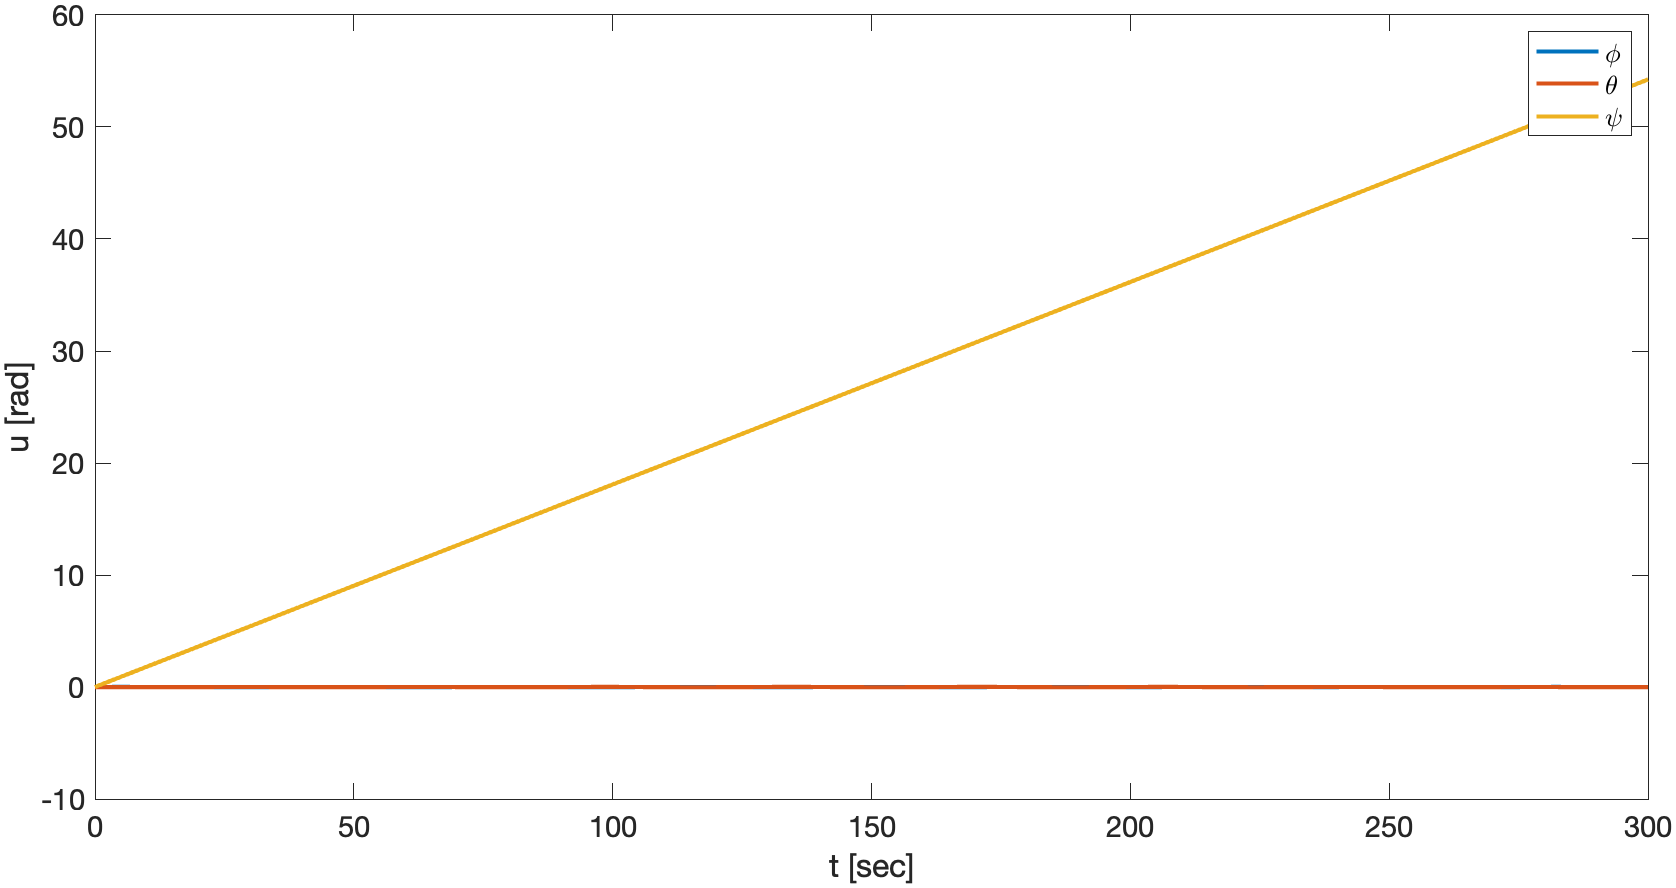
\includegraphics[width = 10cm]{Images/PS4/mom_wheel_intermediate_stability_history_angles.png}
    \caption{Time History of Perturbed 312 Euler Angles Describing Rotation between Inertial and Principal Frame}
    \label{fig:mom_wheel_inermediate_stability_angles}
\end{figure}

\subsubsection{Try to make rotation about another arbitrary axis (potentially relevant to your project) stable
through a generic momentum wheel or rotor.}

Through using the same procedure described in the previous section, we rotated around our body axes selected in Homework 1. This will be relevant for our project as the body axes were chosen to be pointing at important components of the satellite including the instruments, solar array, and antenna. It can be seen that periodic stability about the desired spin axis in the body frame is achieved.

\begin{figure}[H]
    \centering
    \captionsetup{ justification = centering}
    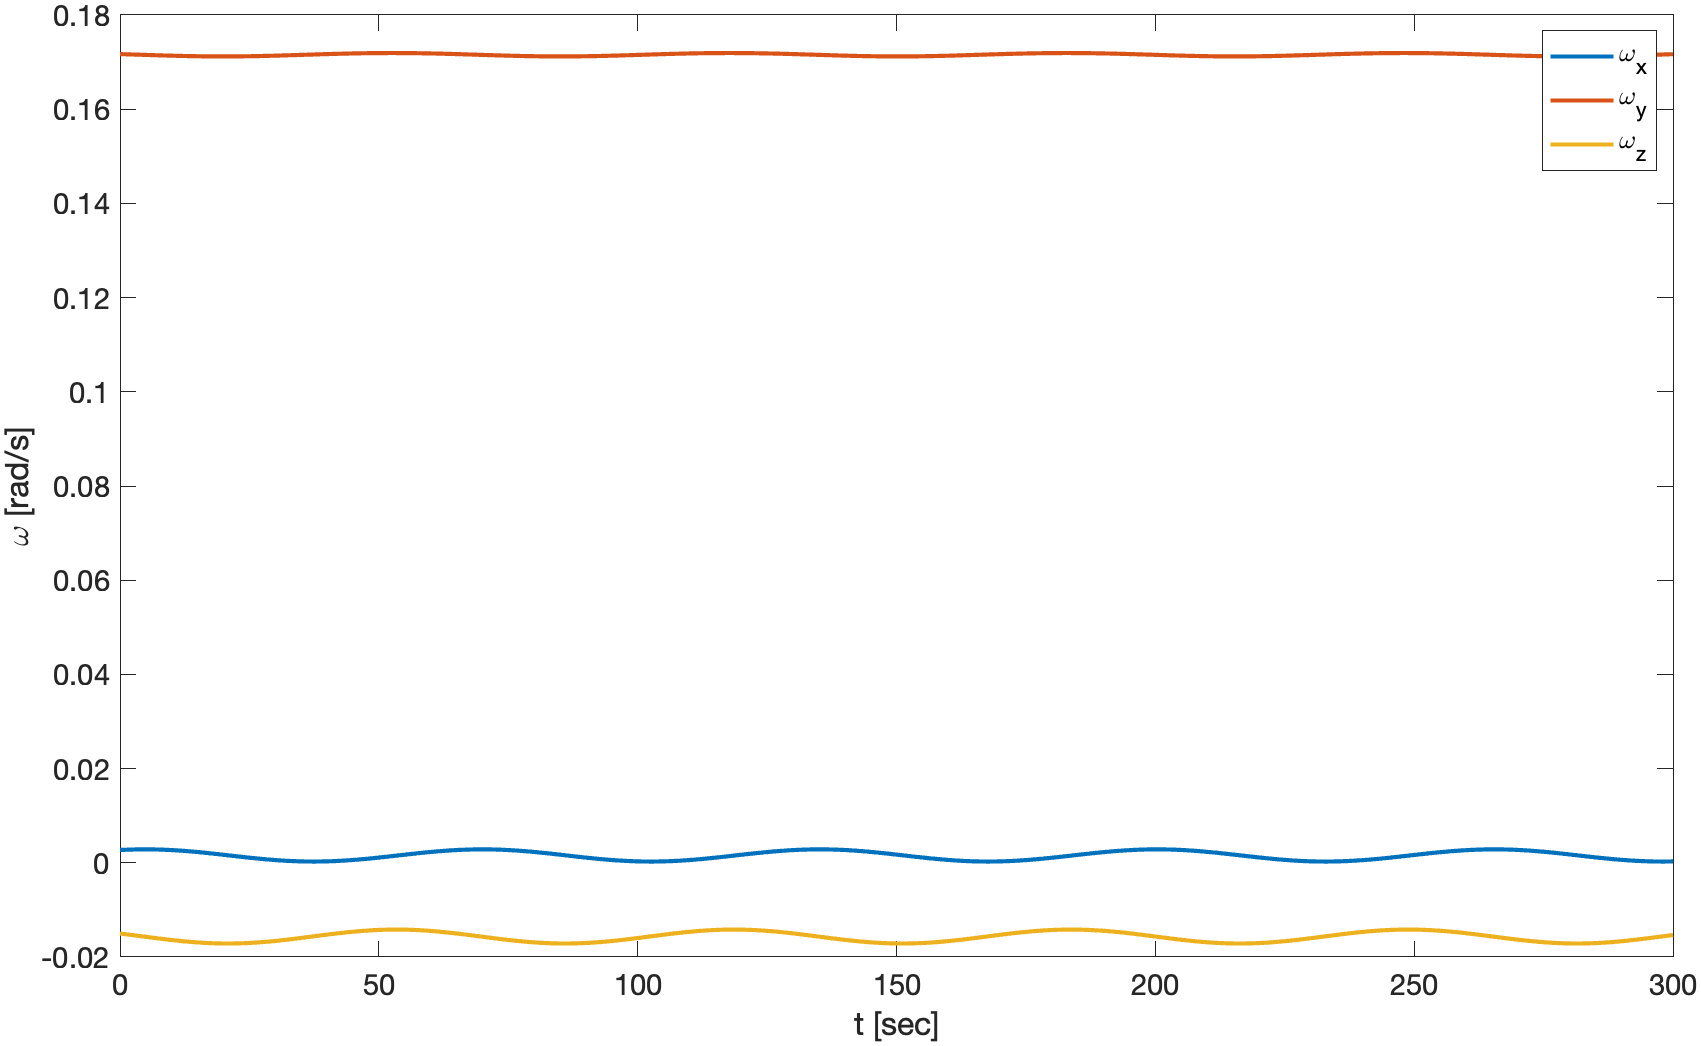
\includegraphics[width = 10cm]{Images/PS4/mom_wheel_mission_stability_history_velocity.png}
    \caption{Time History of Perturbed Angular Velocity Vector Components Expressed in Principal Frame}
    \label{fig:mom_wheel_mission_stability_velocities}
\end{figure}

\begin{figure}[H]
    \centering
    \captionsetup{justification = centering}
    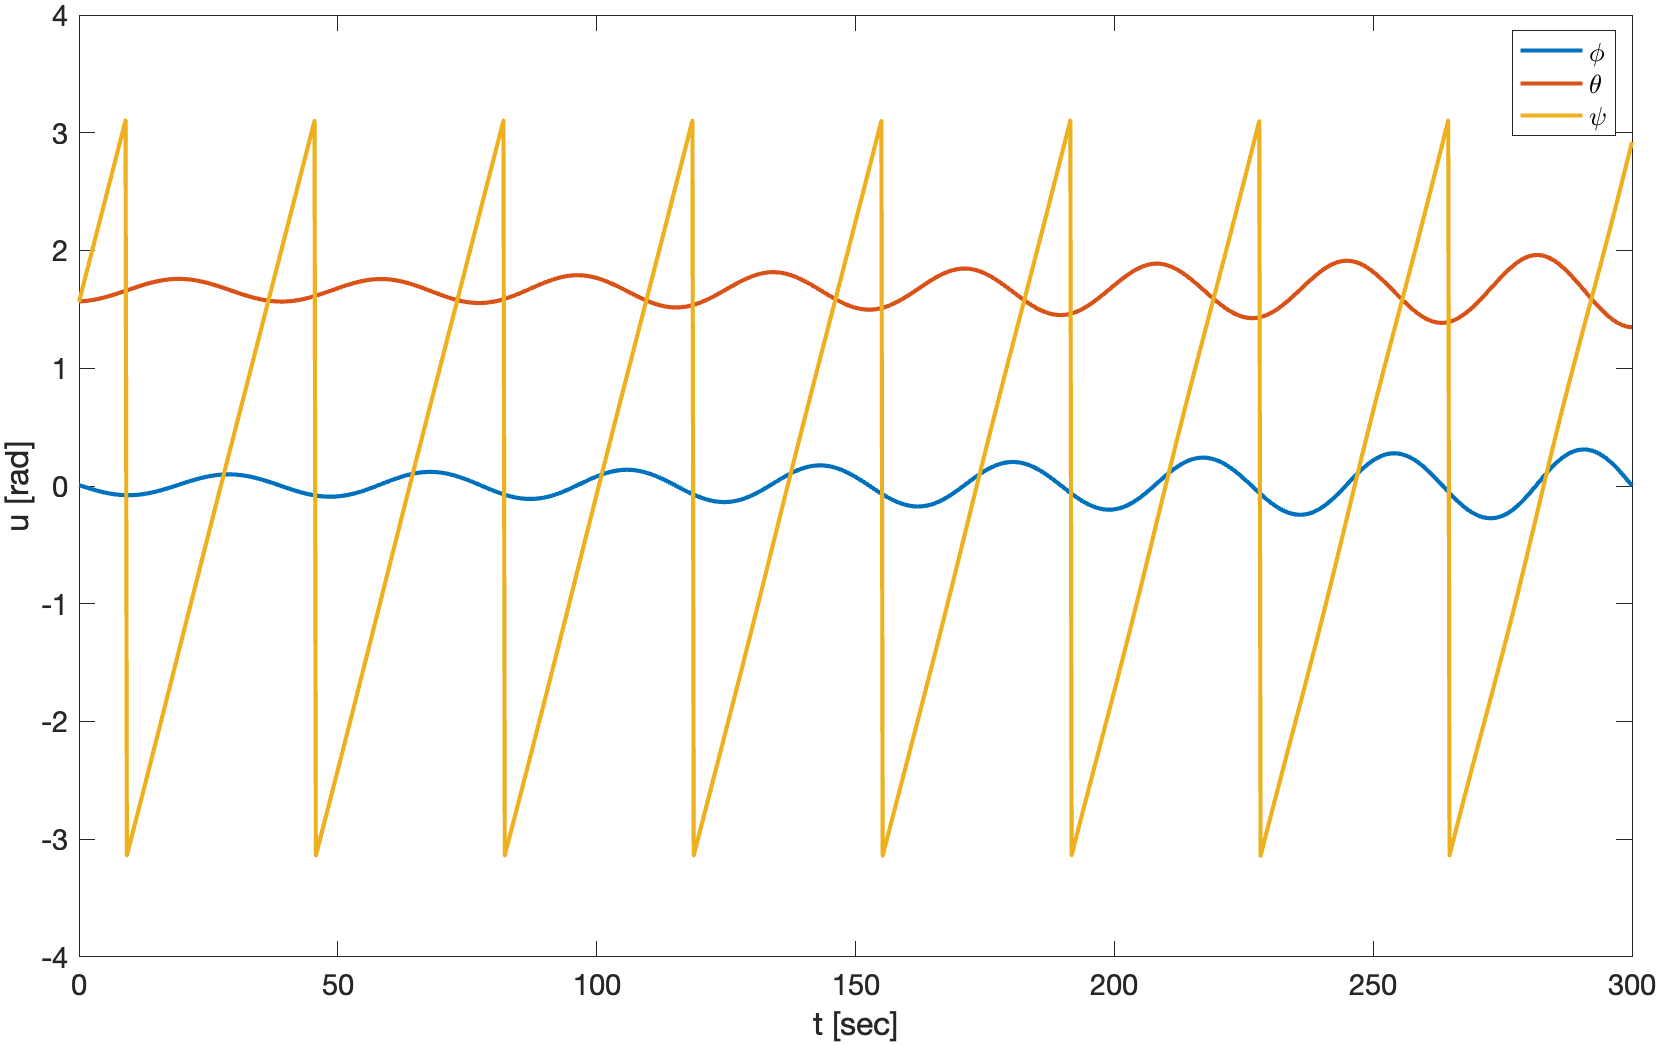
\includegraphics[width = 10cm]{Images/PS4/mom_wheel_mission_stability_history_angles.png}
    \caption{Time History of Perturbed 313 Euler Angles Describing Rotation between RTN and Body Frame}
    \label{fig:mom_wheel_mission_stability_angles}
\end{figure}

\subsection{Problem 4 - Gravity Gradient Torque (Modeling)}

\subsubsection{Remove rotor.}

The simulink model created for this uses variant subsystems to switch between the single and dual rotation configurations very easily.

\subsubsection{Program gravity gradient torque. Feed torque to Euler equations. This is the first perturbation you
model resulting from the interaction of the spacecraft with the environment. Hint: change your orbit
to make gravity gradient significant if that’s not the case.}

Gravity gradient torque is a result of every mass element in the satellite being subject to a slightly different gravitational force due to the small differential of the distance between the distance between each point of the satellite and the center of Earth. While the gravity torque is technically a disturbance, it can be used to stabilize the satellite once it's modeled. 

The torque, $\Vec{M}$, is modeled through taking the gravitation force of Earth ($\mu_{earth} / r^3$) and integrating it over every mass element $dm$ in the satellite. When expressed in the RTN frame, $\Vec{M}$, is shown in the equation below.

\begin{equation}
    \Vec{M} = \frac{3GM}{R^3} \begin{bmatrix}
        0 \\
        I_{rn} \\
        - I_{rt}
    \end{bmatrix}
\end{equation}

Through this, it can be seen that if the principle axes were aligned with the RTN frame, there would be no gravity gradient torque. Finally, expressing $\Vec{M}$ in the principal axes yields the following relationship. 

\begin{equation} \label{eq:grav_gradient_torque}
    \Vec{M} = \frac{3GM}{R^3} \begin{bmatrix}
        (I_z - I_y)c_y c_z \\
        (I_x - I_z)c_z c_x \\
        (I_y - I_x)c_x c_y
    \end{bmatrix}
\end{equation}

This equation was then used to implement the gravity gradient torque in the simulink model shown in the simulink model in Figure \ref{fig:grav_gradient_simulink}.

\begin{figure}[H]
    \centering
    \captionsetup{justification = centering}
    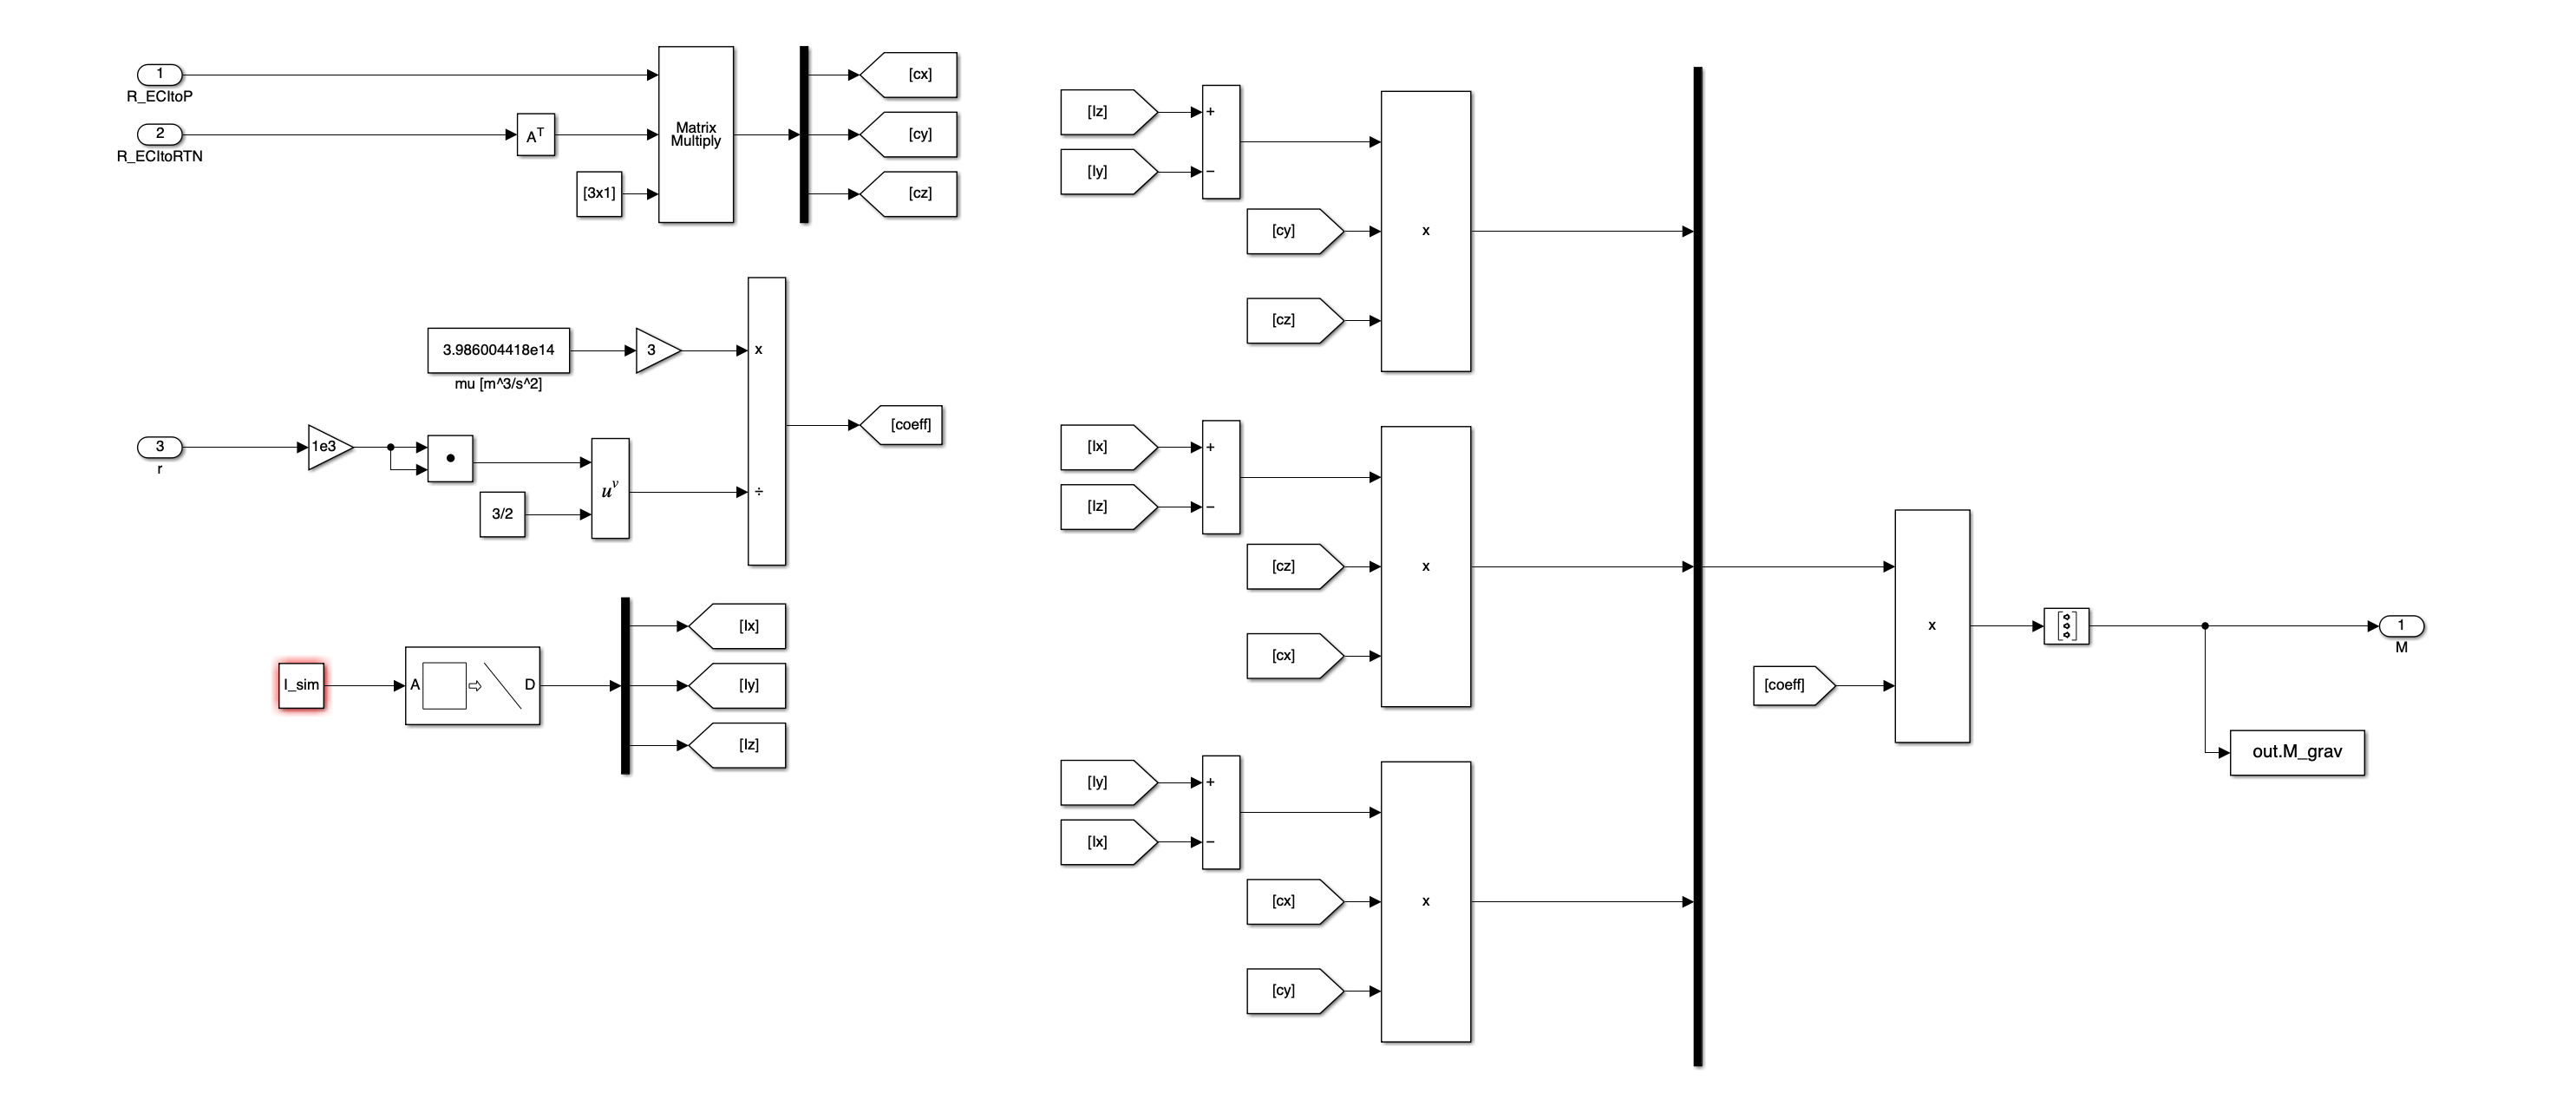
\includegraphics[width = 15cm]{Images/PS4/gravity_gradiant_simulink_model.png}
    \caption{Simulink Model for Gravity Gradient Perturbation}
    \label{fig:grav_gradient_simulink}
\end{figure}

\subsubsection{Verify that the magnitude of the modelled torque is consistent with the orbit and inertia tensor of
your satellite. Hint: use simplified formulas from class on modelling of gravity gradient torque.}

From the simulation results of the simulink model shown above in Figure \ref{fig:grav_gradient_simulink}, the magnitude of $\Vec{M}$ was $10^{-2}$. Since our orbit is nearly circular, we can approximate the radius with the semimajor axis which is set at 7080.6 kilometers. Additionally, the moment of inertias are on the scale of $10^4$ and their differences are on the scale of $10^3$. Finally, the magnitude of the $c$ is $10^{-1}$ Plugging these magnitudes into Equation \ref{eq:grav_gradient_torque}, gives the following magnitude show below.

\begin{equation*}
    ||M|| = \frac{10^5}{(10^3)^3} \cdot 10^3 \cdot 10^{-1} = 10^{-2}
\end{equation*}

\subsubsection{Numerically integrate Euler and Kinematic equations including gravity gradient from initial conditions corresponding to body axes aligned with the orbital frame (RTN). Verify that gravity gradient torque is zero, besides numerical errors. Hint: you may need to simplify the orbit to unperturbed circular to achieve this. Check that initial angular velocity matches mean motion.}

\begin{figure}[H]
    \centering
    \captionsetup{ justification = centering}
    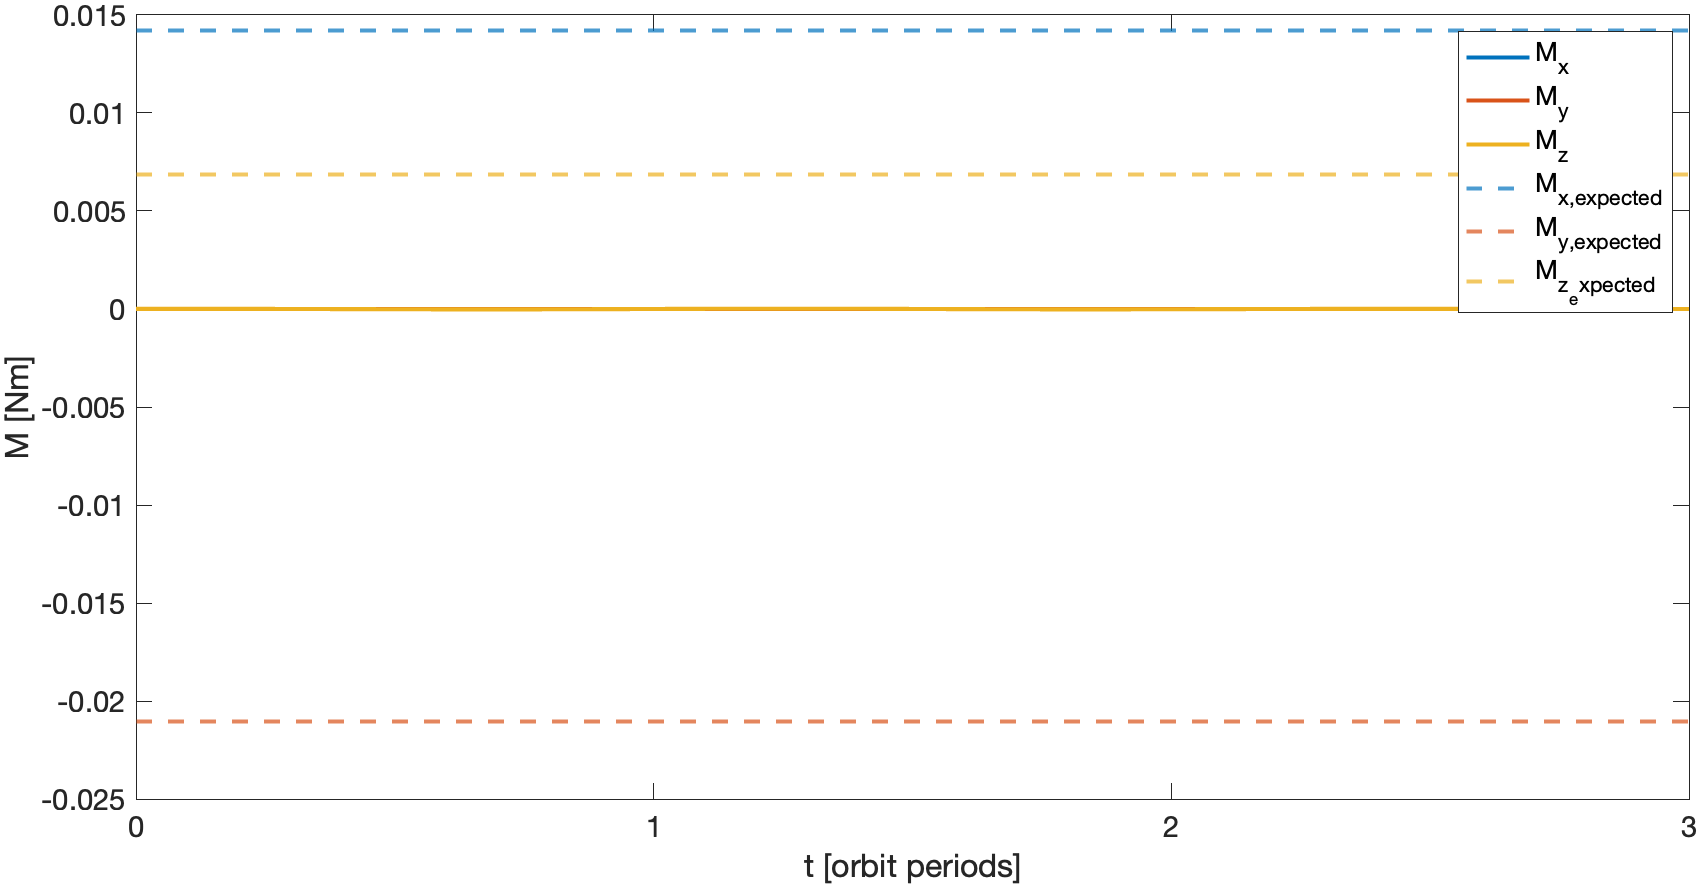
\includegraphics[width = 10cm]{Images/PS4/gravity_torque_RTN_aligned.png}
    \caption{Gravity Gradient Induced Torque Components Represented in Principal Frame Along with Expected Magnitides for Misaligned Torques}
    \label{fig:gravity_gradienet_RTN_aligned}
\end{figure}

As it can be seen in Figure \ref{fig:gravity_gradienet_RTN_aligned}, the expected values of the gravity gradient torque for some chosen $c = \begin{bmatrix} 1/\sqrt{3} & 1/\sqrt{3} & 1/\sqrt{3} \end{bmatrix}^T$ are plotted in dashed lines. Alongside these are the simulated moments for when the satellite principal axes are aligned with the RTN frame. The satellite was given a rotation about its principal z-axis equivalent in magnitude to the mean motion of the orbit. In this case that is 0.0011 radians per second. It can be seen that the torque is either zero or a very small magnitude ($10^{-5}$) for all of the axes. This validates that there are no moments generated when the principal axes are aligned with the RTN frame.

\subsubsection{Numerically integrate Euler and Kinematic equations including gravity gradient from arbitrary initial conditions (e.g., relevant to your project). Plot external torque (3 components w.r.t. time)
and resulting attitude motion (depends on attitude parameterization, add Euler angles for better
geometrical interpretation) over multiple orbits. Comment on results.}

For our project, the relevant initial conditions are the body axes being aligned with a permutation of the RTN frame since our satellite needs to be Earth pointing for several of the sensory and instruments. This is, the rotation from the RTN frame to the desired body axis fram is described as follows where $\vec{v}_b$ is some vector in the body frame and $\vec{v}_{RTN}$ is that vector described in the RTN frame.

\begin{equation*}
    \vec{v}_b = \begin{bmatrix}
        0 & 1 & 0 \\ 0 & 0 & 1 \\ 1 & 0 & 0
    \end{bmatrix} \vec{v}_{RTN}
\end{equation*}

Because the body and principle frames aren't aligned, we would expect non-zero gravity gradient torques in this alignment. The Simulink model shown in Figure \ref{fig:grav_gradient_simulink} was used to propagate the orbits for Figures \ref{fig:gravity_gradienet_mission_aligned}, \ref{fig:grav_mission_velocities}, and \ref{fig:grav_mission_attitudes}.

\begin{figure}[H]
    \centering
    \captionsetup{ justification = centering}
    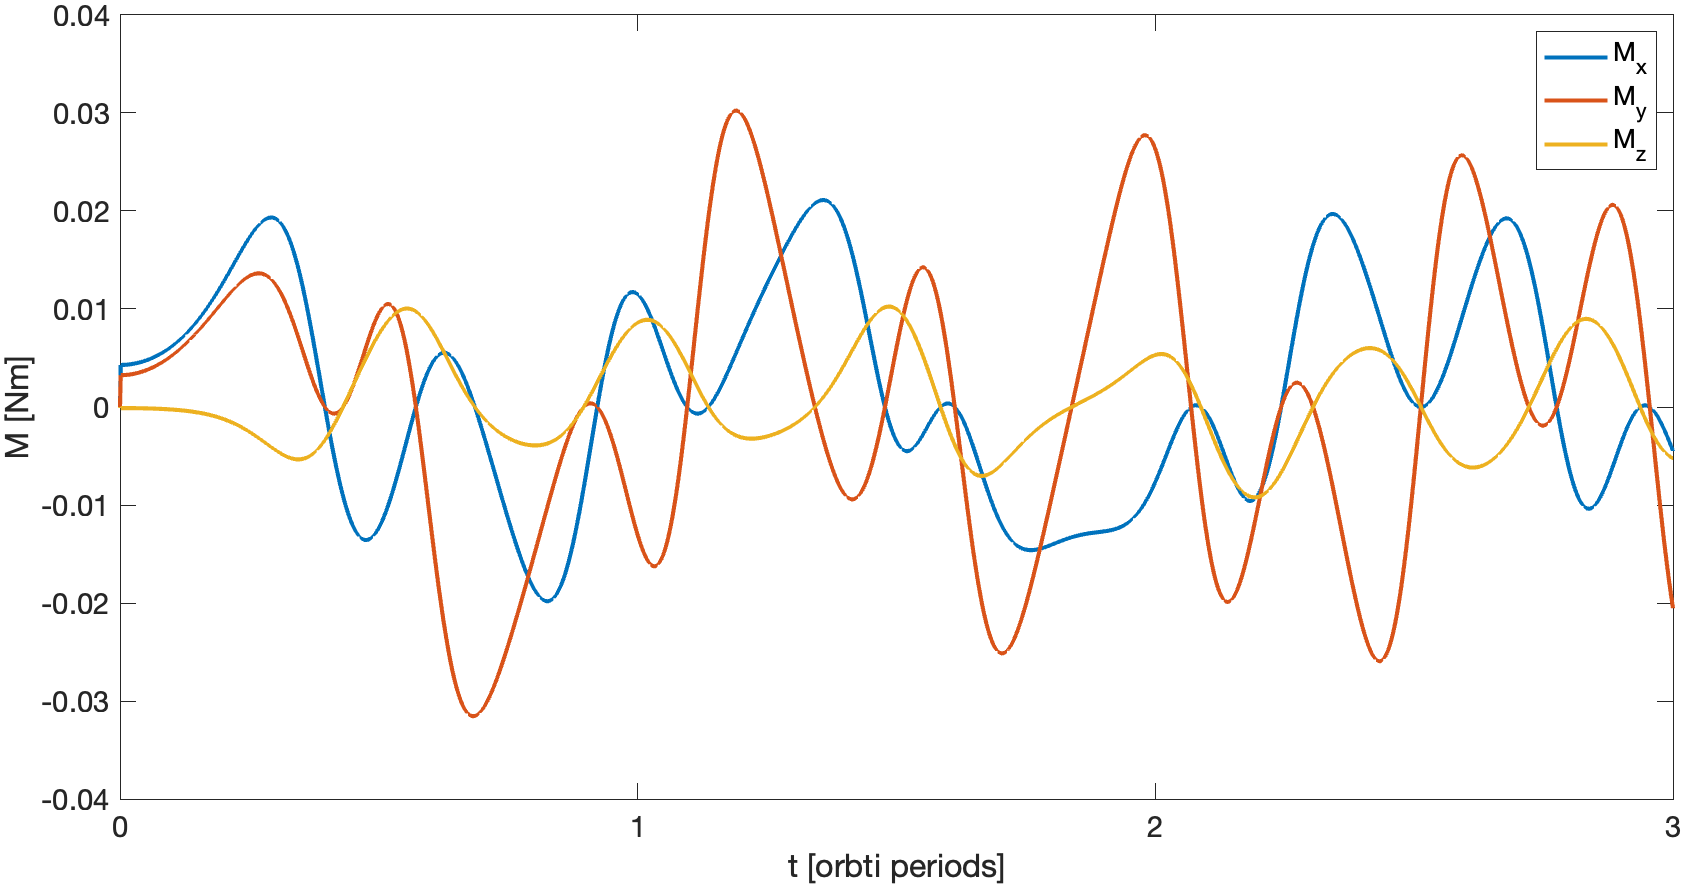
\includegraphics[width = 10cm]{Images/PS4/gravity_torque_mission_aligned.png}
    \caption{Gravity Gradient Induced Torque Components Represented in Principal Frame}
    \label{fig:gravity_gradienet_mission_aligned}
\end{figure}

This expectation is validated in Figure \ref{fig:gravity_gradienet_mission_aligned} through the torques varying in all three of the axis directions.

\begin{figure}[H]
    \centering
    \captionsetup{ justification = centering}
    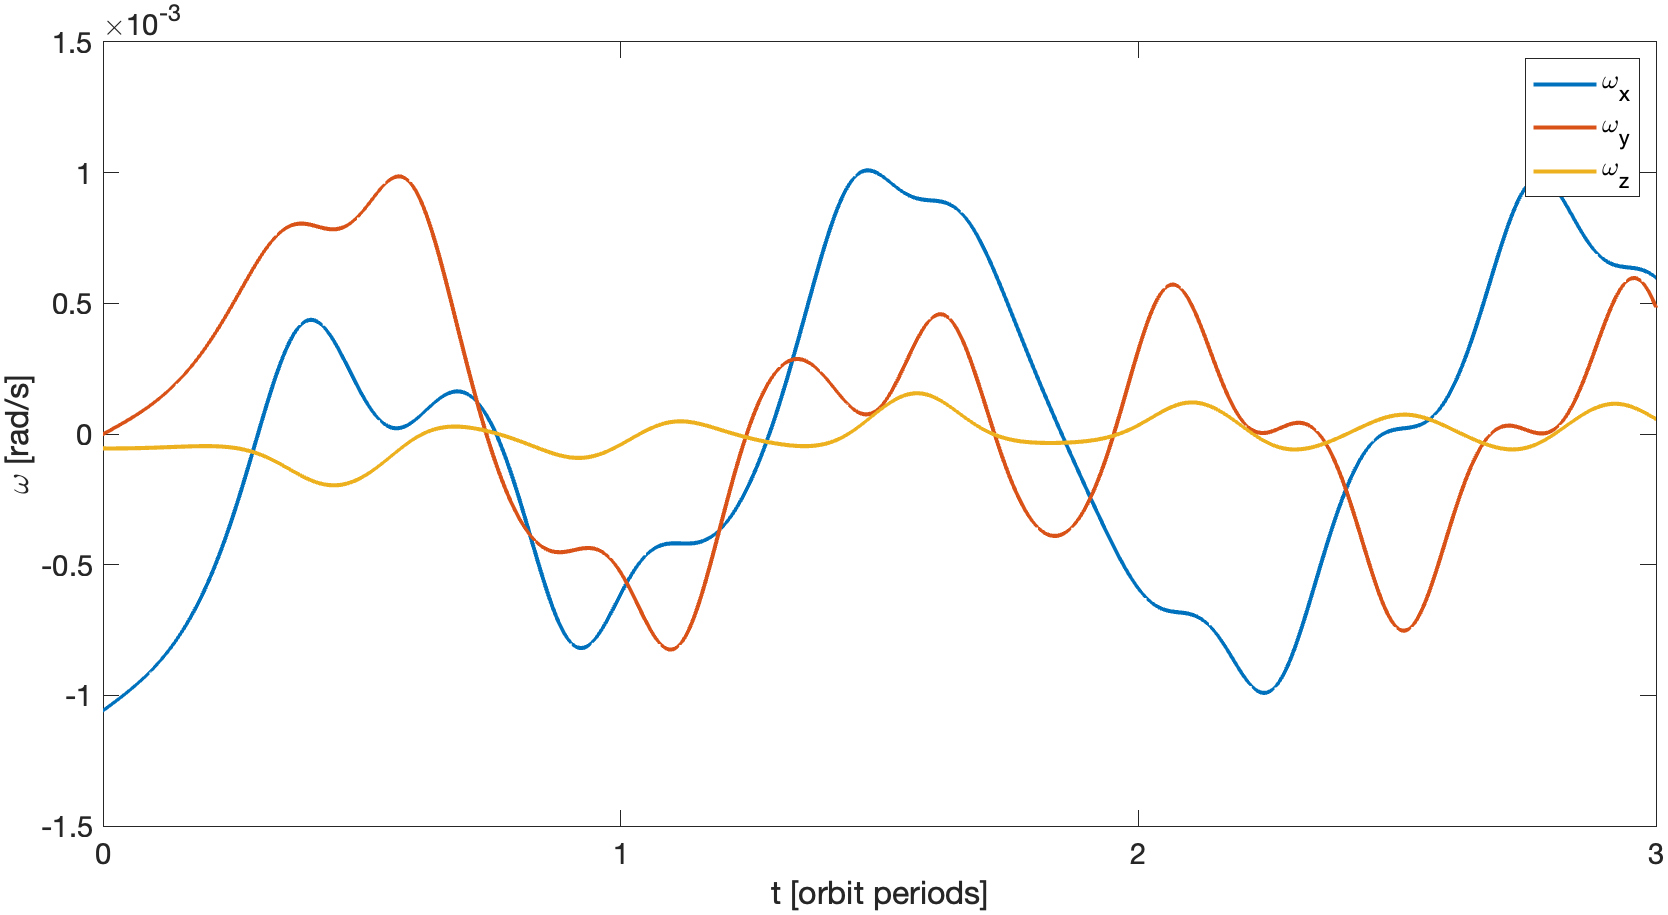
\includegraphics[width = 10cm]{Images/PS4/angular_velocity_under_grav.png}
    \caption{Time History of Angular Velocity Vector Components Expressed in Principal Frame for Mission Aligned Configuration with Gravity Induced Torques}
    \label{fig:grav_mission_velocities}
\end{figure}


\begin{figure}[H]
    \centering
    \captionsetup{justification = centering}
    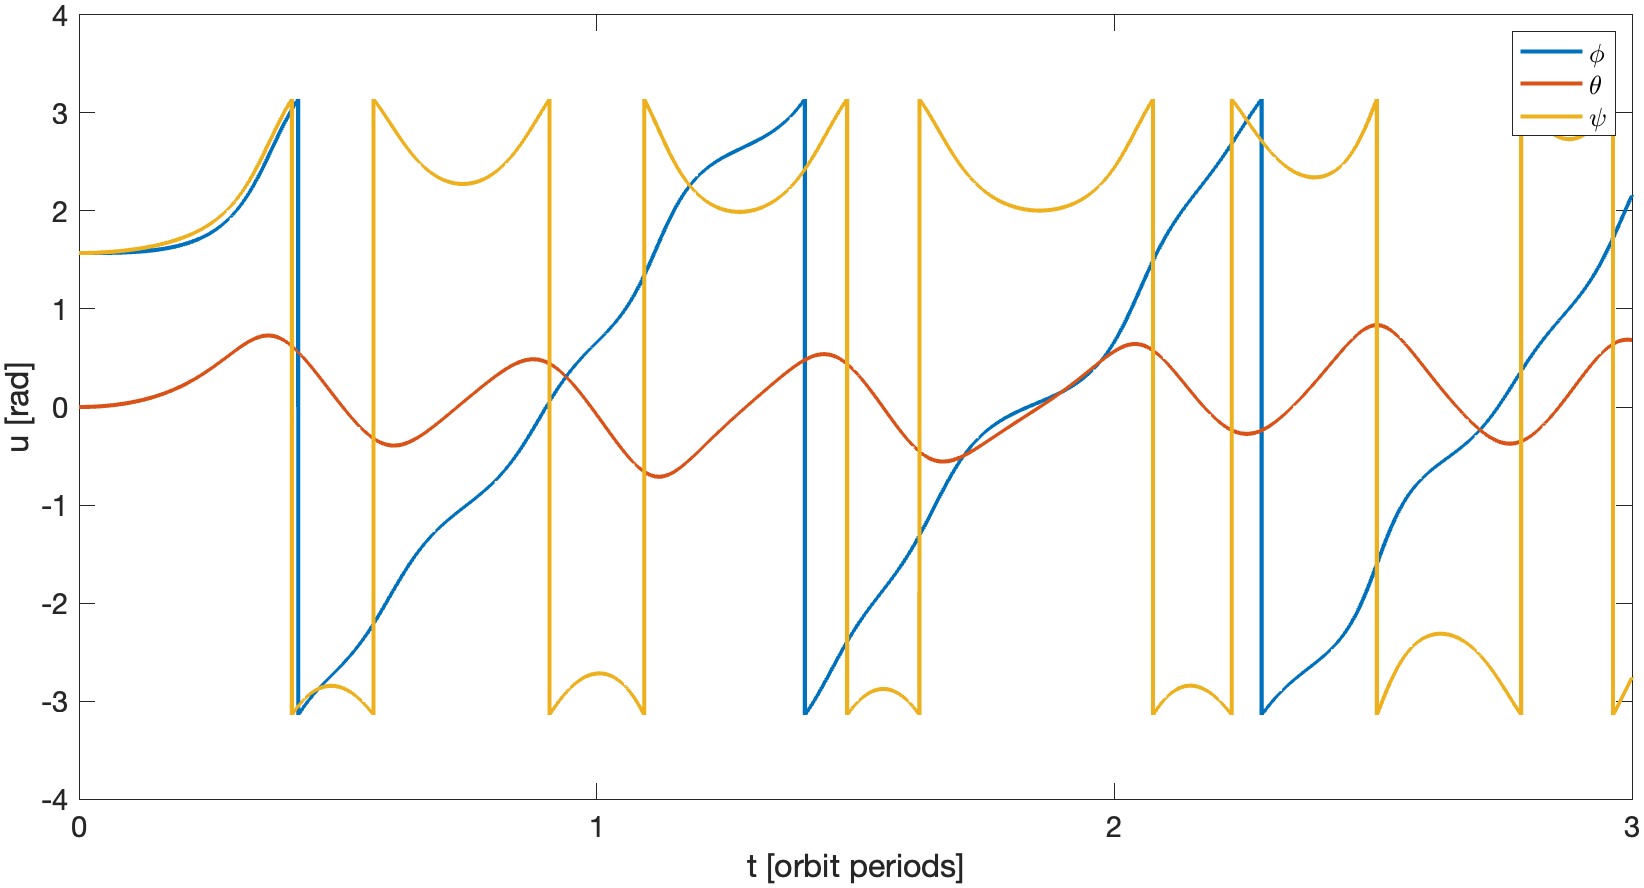
\includegraphics[width = 10cm]{Images/PS4/attitude_under_grav.png}
    \caption{Time History of Perturbed 312 Euler Angles Describing Rotation between RTN and Body Frame for Mission Aligned Configuration with Gravity Induced Torques}
    \label{fig:grav_mission_attitudes}
\end{figure}

The time history of the 312 Euler angles shows that $\phi$ grows at an almost linear rate with only small periodic oscillations. When analyzing the linear portion that gets capped at $[\pi, -\pi]$, it can be seen that  $\phi$ completes one rotation or $2\pi$ radians for every orbital period. This aligns with what should theoretically happen as the radius vector in the RTN frame completes an entire sweep in that amount of time. The time history also shows that $\psi$ oscillates around $\pi$ radians (a little hard to see since the angles are defined to always stay between $[\pi, -\pi]$) and $\theta$ oscillates around 0 radians. This also makes sense since large effects from the RTN frame aren't shown in $\psi$ and $\theta$ and instead their oscillations come from the gravity gradient torque. Finally, it can be noted that the periods of the oscillations remain constant for the entire simulation.
